\chapter{Interpretation and comparison of results}
The previous sections showed that all simulated solar power plants are able to cover the predicted load curve for more than \SI{90}{\percent} over the year using specified configurations. To describe this in a wildly-used indicator, all simulated power plants are reaching a CF of about \SI{73.1}{\percent} in these specified scenario. The selected power plant configuration of each technology to cover the prescribed load at the lowest LCOE are summarized in Table~\ref{tbl: summaryresult}.
\begin{table}[!htbp]  
  \centering
	\begin{tabular}{ p{3.0cm} C{3.6cm} C{3.6cm} C{3.6cm} } 
	\hline	
&\multicolumn{3}{c}{\textbf{Selected configuration to cover the predicted load}}\\

\textbf{Type} & \textbf{$\geq$~\SI{70}{\percent}} & \textbf{$\geq$~\SI{80}{\percent}} & \textbf{$\geq$~\SI{90}{\percent}} \\ \hline \hline
CR power plant 	& SM:~2.0 \& TES:~10~h	& SM:~2.5 \& TES:~10~h & SM:~3.0 \& TES:~14~h \\
PTC power plant	& SM:~3.0 \& TES:~10~h	& SM:~3.5 \& TES:~12~h & SM:~5.0 \& TES:~12~h  \\
PV power plant	& PVM:~2.2 \& EES:~4~h	& PVM:~2.6 \& EES:~5~h & PVM:~2.8 \& EES:~7~h \\
\hline
\end{tabular}
\caption[Summary of selected solar power plant configurations to reach the target load covering at lowest LCOE.]{Summary of selected solar power plant configurations to reach the target load covering at lowest LCOE.}\label{tbl: summaryresult}
\end{table}

\section{Comparison of performance results}
The summary in the Table shows, that the expenditure in technical and therefore also in economic terms are quite different between the technologies to reaching higher load curve coverings. When comparing the rising multiple of the design point of the solar power plants to reach a higher amount of annual load covering it seams that the effort is quite different between the technologies. When comparing the necessary growing multiple to the design point of the power plants to reach higher annual load curve covering it seams obviously that the effort of the PTC technology rises at most. The PTC power plant needs a about five-times larger solar field (SM of 5.0) in reference to the design point to cover \SI{90}{\percent} of the predicted load over the year. This is particular high, especially in comparison to the SM of the CR power plant system at the same design point which needs just a three times larger heliostat field. As it was shown before in Section~\ref{sec.resultsPTC} the high effort of the PTC technology to reach high load curve covering values is based on the optical efficiency loss of the solar field at low irradiation angle through the cosine effect. The optical efficiency loss through the cosine effect affects also the CR system, but thanks to the two-axis tracking of the heliostats is the influence comparatively small. 

Both solar fields are highly over scaled to producing enough thermal power for the whole day in winter times, thereof it results that they need to reduce the field optical focus fraction in summer times significantly. The average field optical focus fraction of both selected CSP technologies for December are shown in Figure~\ref{FocusFraction}. The December average shows that more than \SI{60}{\percent} of the CR heliostat field is defocused from 13:00 to 15:00 and also the half solar field of the PTC plant needs a focus fraction. This leads to enormous unused capacities of the CSP fields. 
\begin{figure}[!htbp]
        \centering                
        \begin{subfigure}[b]{0.5\textwidth}
                \centering
                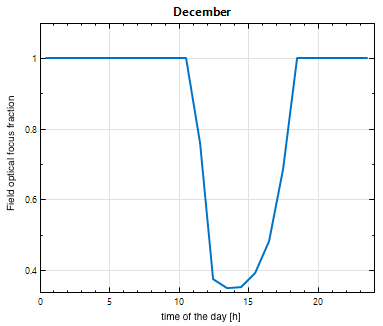
\includegraphics[width=1\textwidth]{FIG/FocusFraction/DecemberCR}
                \caption{Average CR heliostat field focus fraction in December at a SM of 3.0 and 14~h of TES.}\label{DecemberCR}
        \end{subfigure}%
        ~
        \begin{subfigure}[b]{0.5\textwidth}
                \centering
                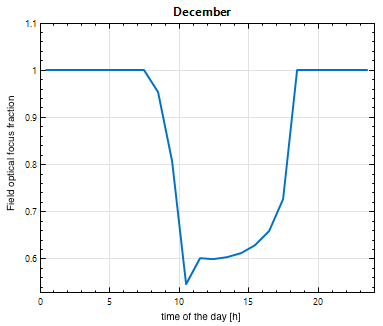
\includegraphics[width=1\textwidth]{FIG/FocusFraction/DecemberPTC}
                \caption{Average PTC SCA field focus fraction in December at a SM of 5.0 and 12~h of TES.}\label{DecemberPTC}
        \end{subfigure}
        \caption[Average field optical focus fraction in December of for 90~\% load curve covering configurated CSP technologies.]{Average field optical focus fraction in December of for 90~\% load curve covering configurated CSP technologies.}\label{FocusFraction}
\end{figure}

The designed PV power plant is fixed orientated and doesn't track the sun, nevertheless for reaching a covering of 90~\% of the prescribed load over the first year the PV power plant needs a lower multiple of the design point than the other two solar power plants. This mainly comes from the characteristics of the PV system by using GHI instead of DNI. Upington has a huge amount on direct irradiation but also cloudy days with diffuse irradiance (see Figure~\ref{DHI-DIF}). Therefrom the PV power plant needs a lower multiple of the PV system and a smaller storage compared to the CSP power plants. Also the surplus net output of the simulated PV power plants is just about 2.2 and 5.5~\% over the year. Compared with the defocused solar field capacities of the CSP plants this is a very small value.

\begin{figure}[htbp]  
\centering
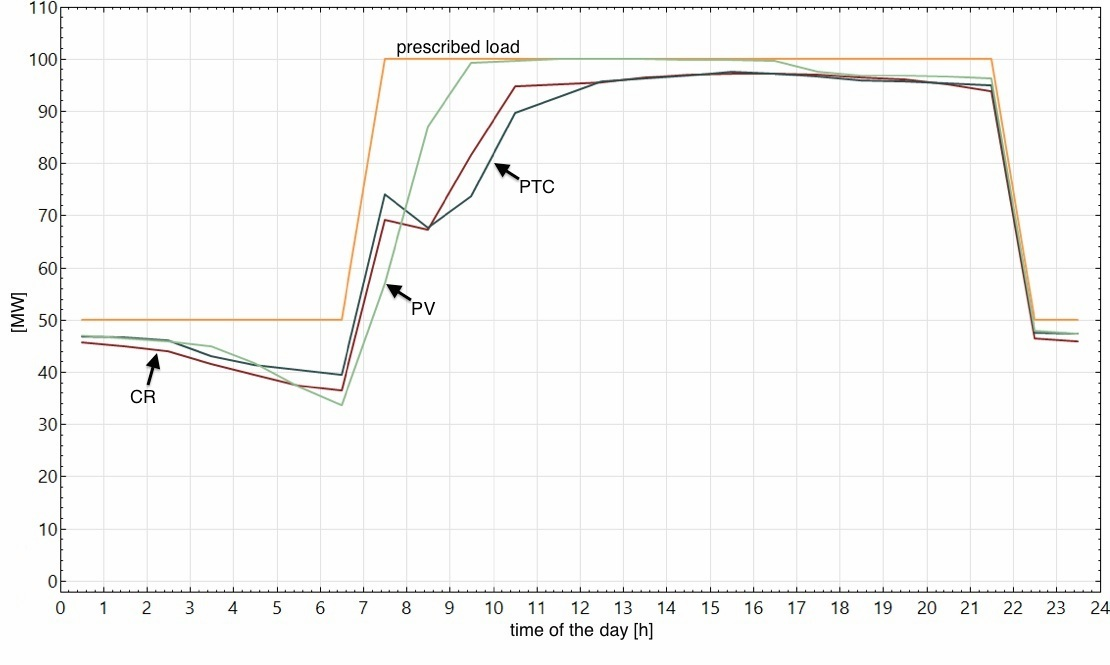
\includegraphics[width=0.8\linewidth]{FIG/90_annual_profil}
\caption[Annual average load profile of selected PV power plant configurations.]{Annual average load profile of selected PV power plant configurations.}\label{90_annual_profil}
\end{figure}
The annual average load profiles of the in Table~\ref{tbl: summaryresult} specified  power plant configuration over 90~\% load covering are compared in Figure~\ref{90_annual_profil}. It can be seen that they profiles of the three solar power plant are relatively equal. But it is noticeable that the PV plant can fully cover the load from 10:00 to 16:00 over the full year. Compared to are the annual average net energy outputs of the CSP plants just below, but can't cover the load like the PV power plant. This mainly comes from the not exactly configurable turbine power output control, which settings was described in the respective simulation design sections. It can be assumed that under real conditions a steam Rankine power output control is working far more accurate. 

As the line chart shows all simulated solar power plants are having there main leak in supply during the morning hours. But this mainly comes from the weaker power generation during the winter time, where the irradiation amount and angle of sunlight radiation is lower. Basically can be said that all three here shown solar power plant covers the load almost continuously over the year, but during the mentioned time during the winter all solar power plants coming to standstill. This can also be seen in the net power output heat maps of Figure~\ref{Heatmap}. The Figures describes the net power output of the selected simulated solar power plants at any hour of the simulated year. It just shows the net power output which is covering  the prescribed load and no surplus net power. It describes therefore the values of the annual average load profile from the line chart above more in detail. The power reduction during the night time from 22:00 to 7:00 is clearly visible in the heat maps. Also can be seen, that all solar power plants has interruptions in supply on various days in the year which leads from low direct or global irradiation at days of bad weather. 

\begin{figure}[!htbp]
        \centering   
        \begin{subfigure}[b]{1\textwidth}
                \centering
                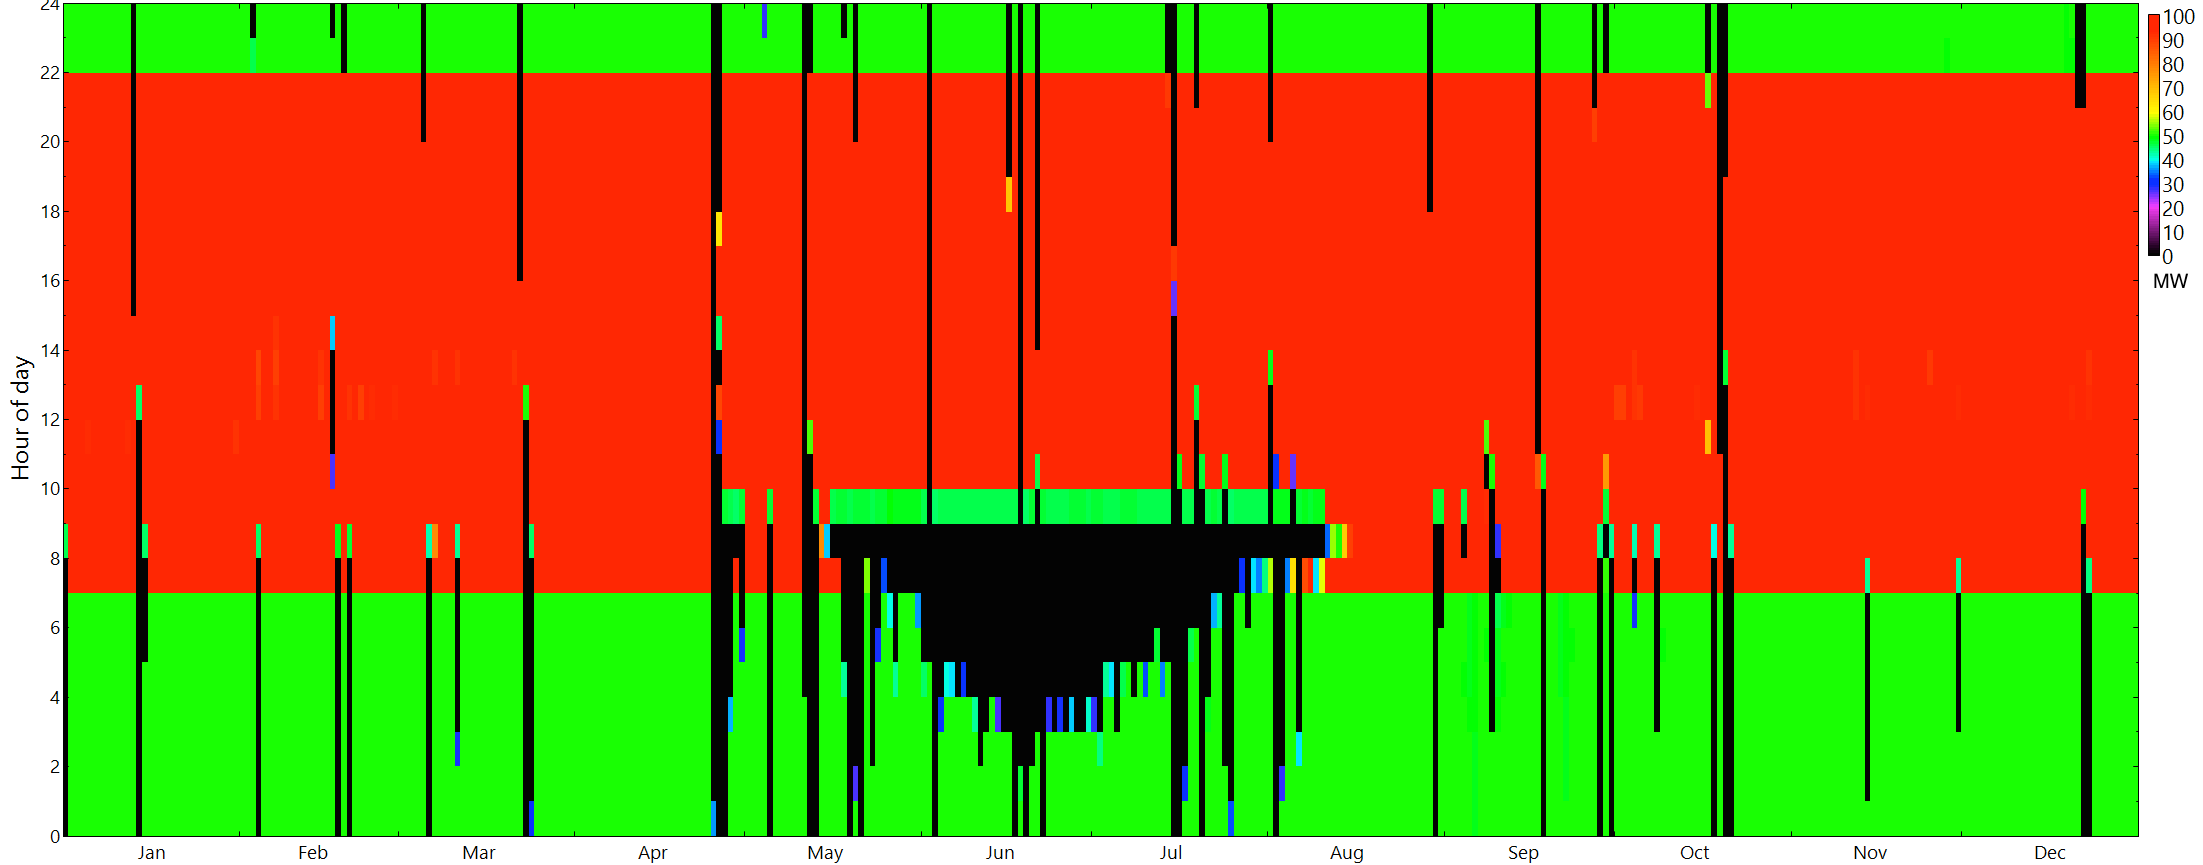
\includegraphics[width=1\textwidth]{FIG/HeatmapCR}
                \caption{CR with a SM of 3.0 and 14~h of TES.}\label{HeatmapCR}
        \end{subfigure}
        
\par\medskip % Linebreak

        \begin{subfigure}[b]{1\textwidth}
                \centering
                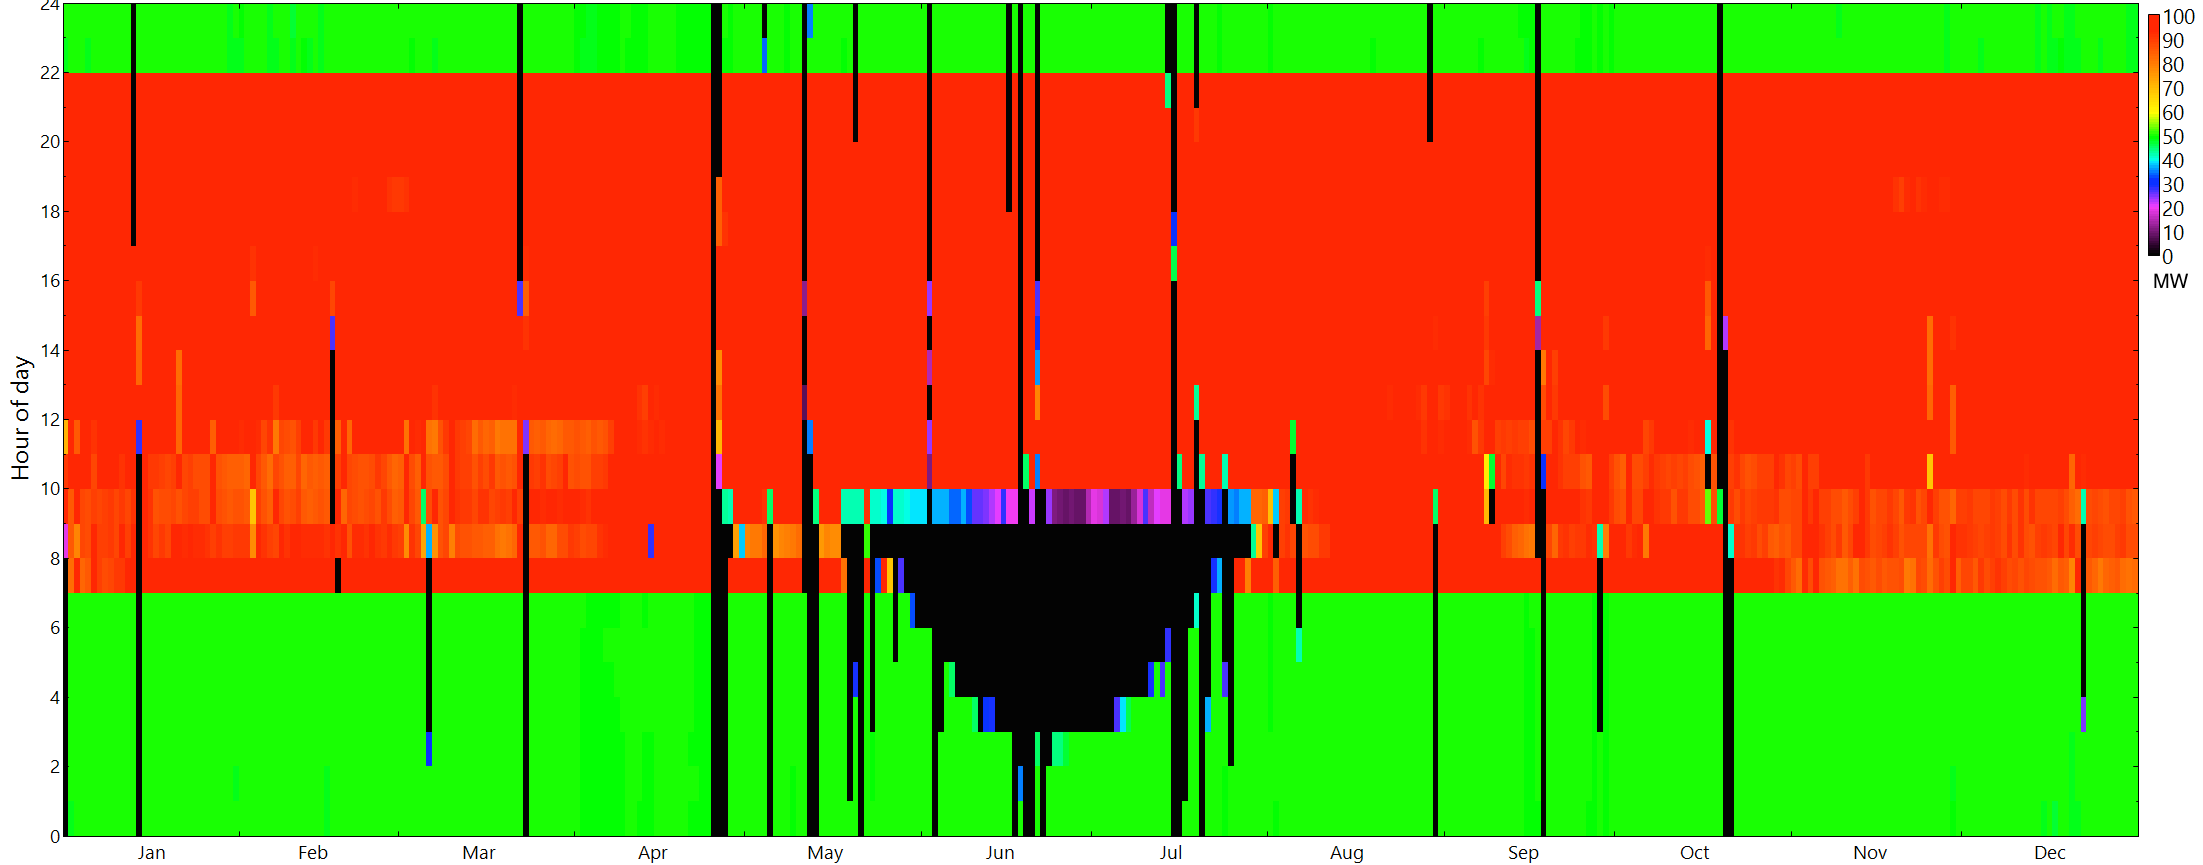
\includegraphics[width=1\textwidth]{FIG/HeatmapPTC}
                \caption{PTC with a SM of 5.0 and 12~h of TES.}\label{HeatmapPTC}
        \end{subfigure}
        
\par\medskip % Linebreak     
           
        \begin{subfigure}[b]{1\textwidth}
                \centering
                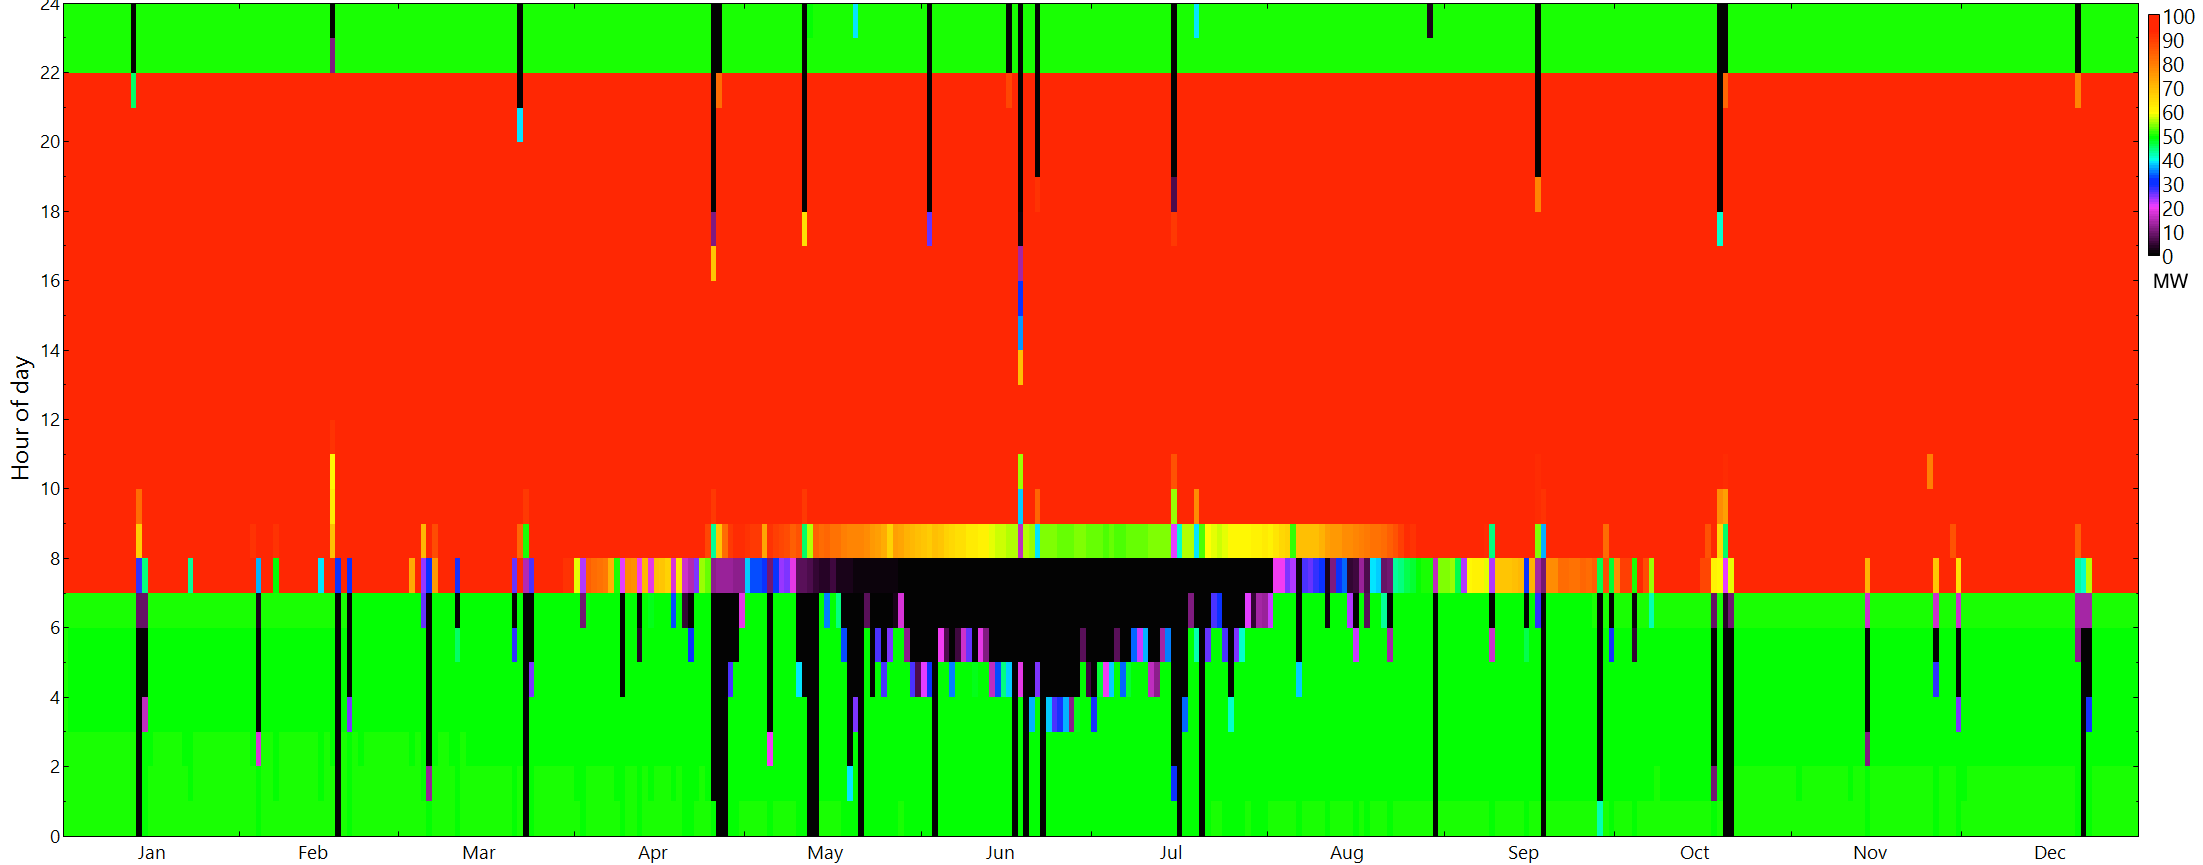
\includegraphics[width=1\textwidth]{FIG/HeatmapPV}
                \caption{PV with a PVM of 2.8 and 7~h of EES.}\label{HeatmapPV}
        \end{subfigure}
        \caption[Net power output to predicted load from selected solar power plants shown as heat map over the simulated year.]{Net power output to predicted load from selected solar power plants shown as heat map over the simulated year.}\label{Heatmap}
\end{figure}
At first it is obviously when comparing the heat maps that at the time of winter solstice all power plants coming to standstill in the morning hours. When taking a view at the stating time of the power plants during that time it can be noted that the PV power plant starts about one hour earlier than the other two plants. On one site this leads from the for the PV system usable diffuse share of the GHI at dawn and on the other site from the set power block starting up time of 30 minutes for both CSP plants. It can also be noted, that the PTC system is starting with less power output then the CSP system at these time of the year.

The heat map of the PTC shows a slightly lower power output during the time from 8:00 to 12:00 in summer time. This leads from the above mentioned power output control, but also from high parasitic consumer of the power plant during that time. When taking an eye on the power output of the PV power plant it can be said that the plant fully covers the predicted load over the year from 11:00 to 13:00.

\section{Electricity cost results and outlook}
The comparison shows that all solar power plants are able to cover the predicted load with there individual configured systems. But the cost effort is different between the systems which is also reflected in the investment costs and therefrom in the LCOE. Figure~\ref{LCOEcomparision} summarizes the the LCOE calculation results of the selected solar power plants from Table~\ref{tbl: summaryresult} and compares them with each other and with public projection ranges. 

\begin{figure}[htbp]  
\centering
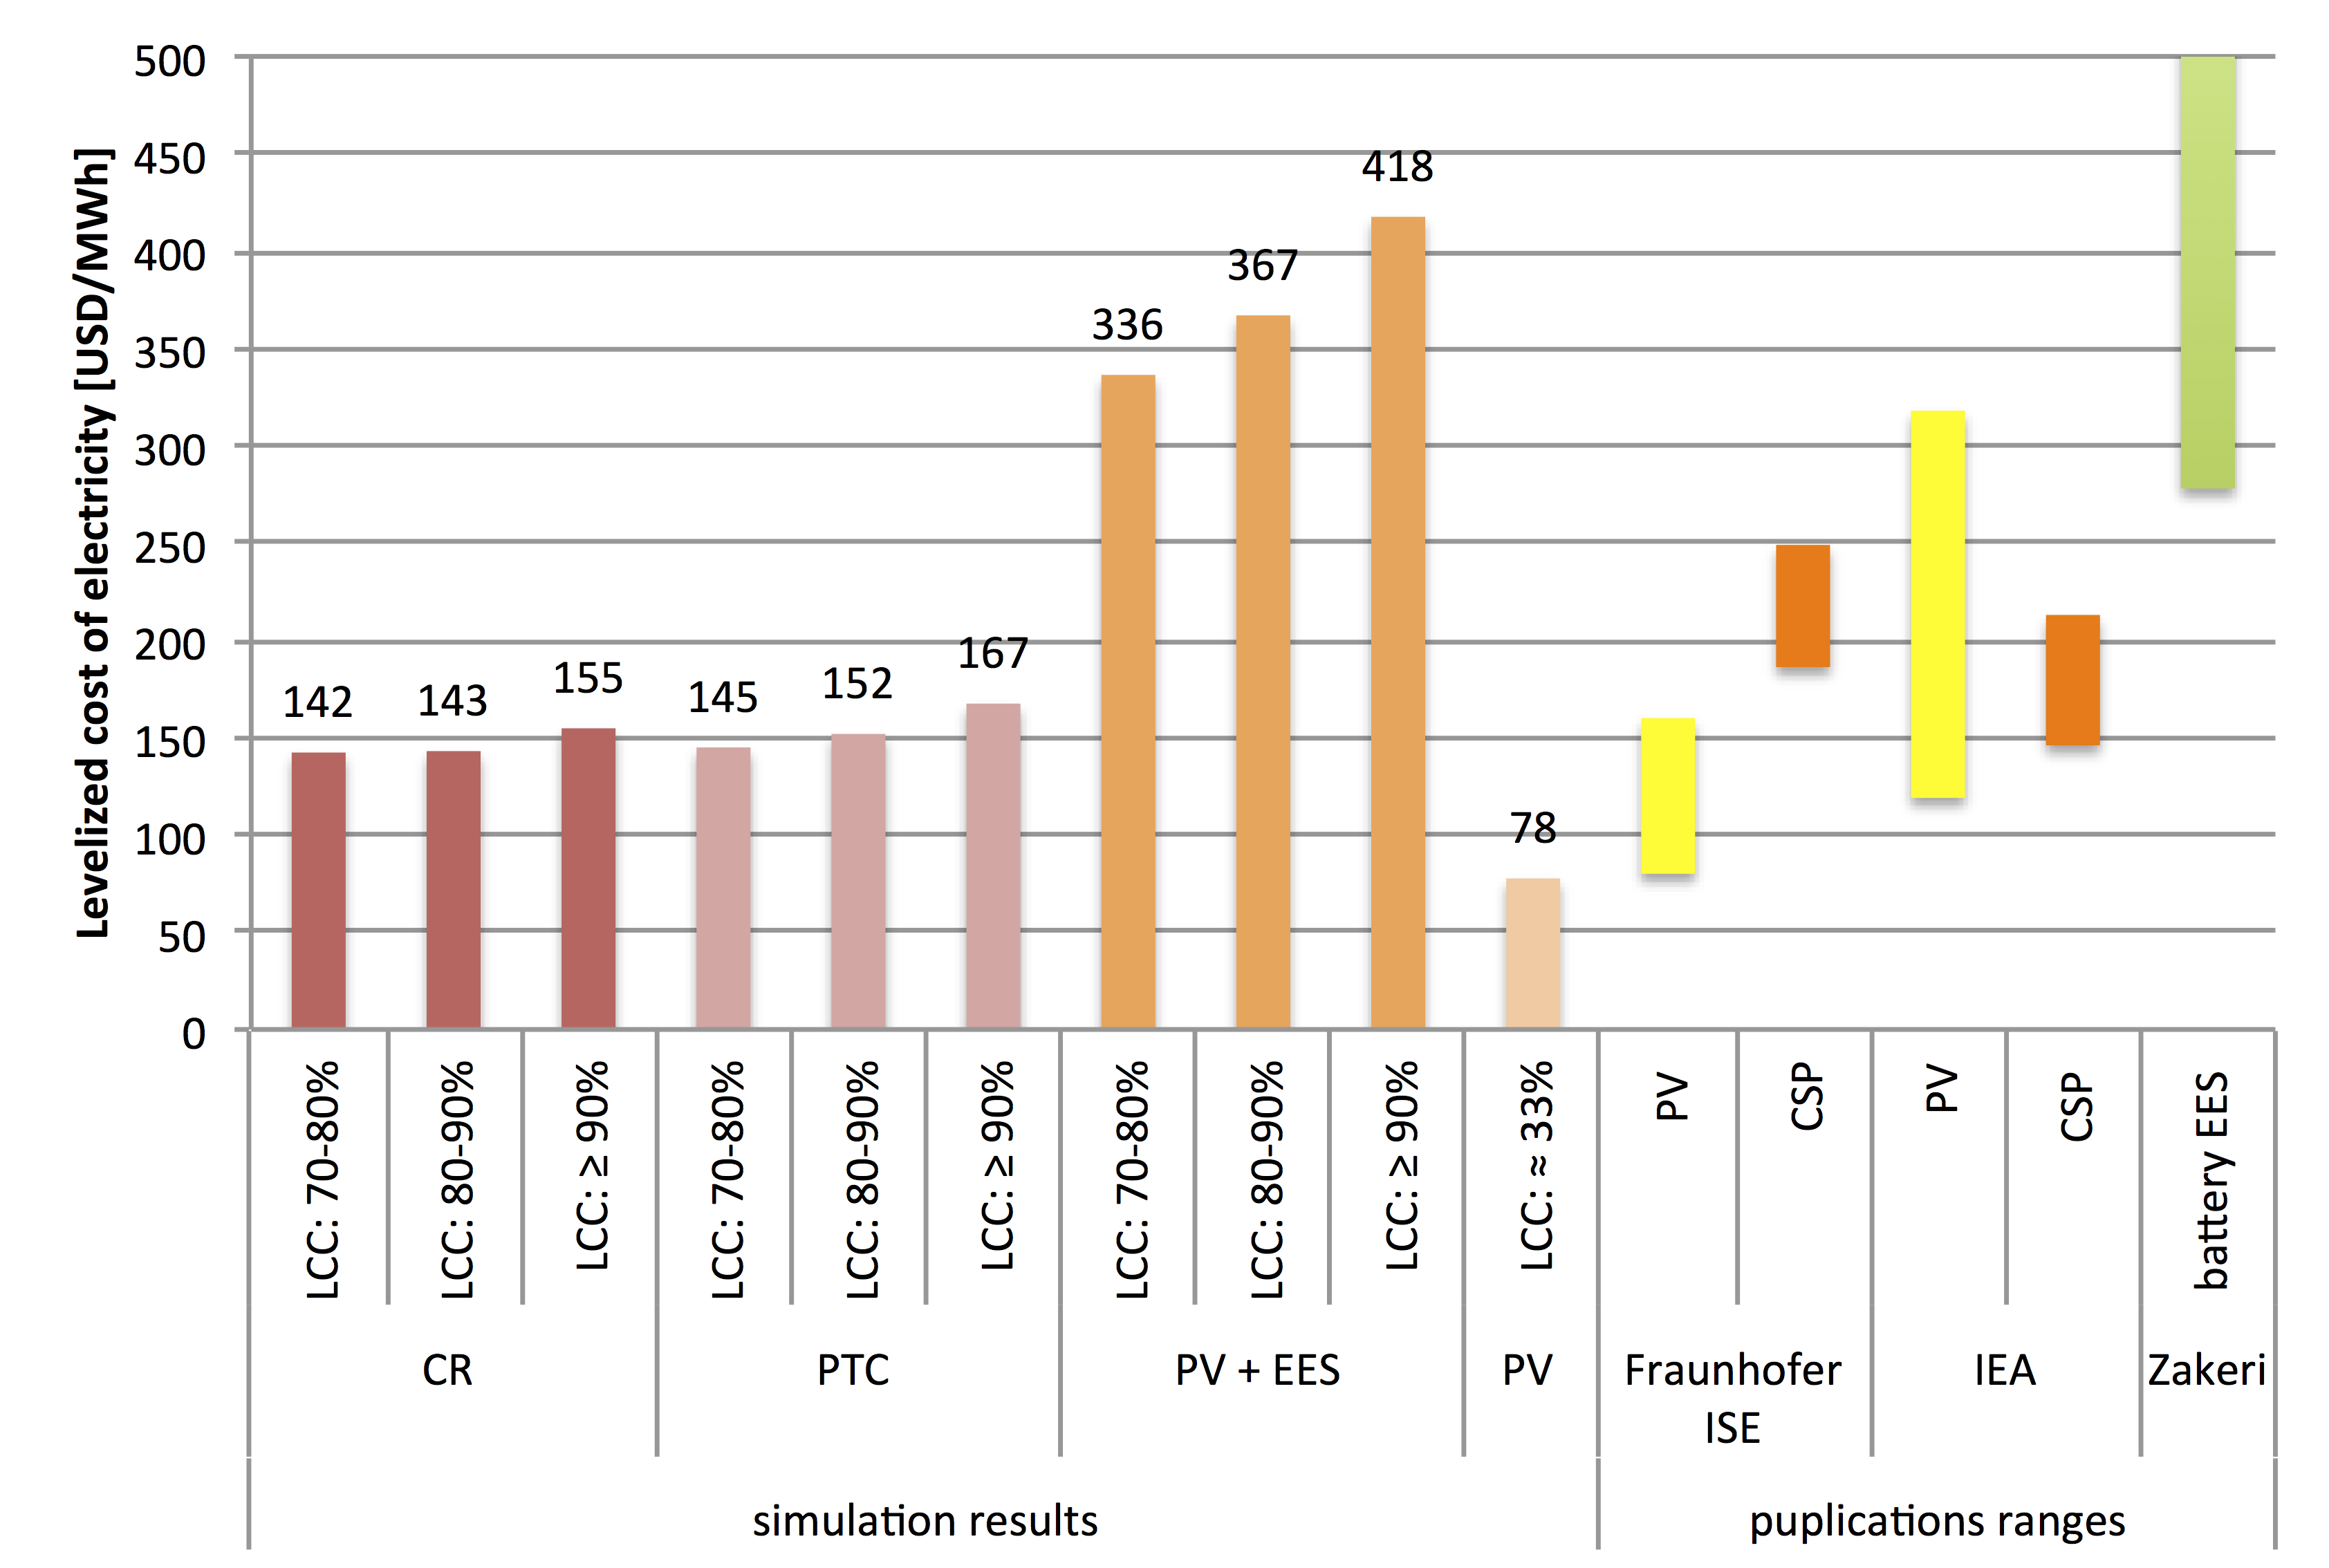
\includegraphics[width=1\linewidth]{FIG/LCOEcomparision}
\caption[Summary of calculated LCOE results of simulated solar power plants compared with public projections.]{Summary of calculated LCOE results of simulated solar power plants compared with public projections.}\label{LCOEcomparision}
\end{figure}
Overall for all simulated solar power plants can be said, that with the higher load covering rate also the LCOE increases.

It can be seen that the PV system without EES reaches with \SI{78}{USD/MWh} the lowest LCOE of the simulated power plants, but therby it covers the load curve just about \SI{33}{\percent} over the first year. In comparison with other projections can be seen that the PV system in Upington reaches an low LCOE result. The Fraunhofer ISE institute names the LCOE range\footnote{PV system LCOE result rages from \SIrange{60}{120}{EUR/GWh} by using a WACC of \SI{4.7}{\percent}  \cite{FraunhoferISE2013} at an avarage exchange rate in 2013 and 2014 of \SI{1.33}{USD/EUR} \cite{StatistaGmbH2015}.} for PV systems in 2013 between 80 and \SI{160}{USD/GWh} for areas with a GHI of \SIrange{1450}{2000}{\kilo\watt\hour\per\square\metre\per\year} \cite{FraunhoferISE2013}. When including the higher GHI value of Upington (\SI{2280}{\kilo\watt\hour\per\square\metre\per\year}) and the lower assumed invest costs than in 2013 the calculated LCOE seams realistic. The International Energy Agency (IEA) published the LCOE values for the year 2015 in there annual report of "Tracking Clean Energy Progress 2014" more conservative \cite{IEA2014c}.

The lowest LCOE calculation results of the simulated solar power plants which covers more than \SI{90}{\percent} of the predicted load curve has the CR power plant with about \SI{155}{USD/MWh}. The CR power plant in generally reaches the lowest LCOE values while having a high load curve covering rate. Also the LCOE result of the PTC power plant is with \SI{167}{USD/MWh} relatively low. When comparing this values with the projections of Fraunhofer ISE institute from 2013 the results looking quite optimistic. But when comparing with the electricity cost range from the IEA publication the CSP simulation results seams realistic.

The LCOE calculation results of the simulated PV system with adapted EES is by far the most expansive solution for suppling the prescribed load. The lowest LCOE for reaching \SI{90}{\percent} LCC is more than twice that high than from the CSP options. For the comparison also must be remembered, that the costs of the EES storage part was assumed extremely low in comparison with the average marked price (Page~\pageref{SUBSUBPVFinancialparameter}). But when using other optimistic LCOE calculations of battery EES the result seams realistic. There are optimistic puplications calculated a LCOE of a battery EES with about \SI{200}{USD/MWh} pure storage costs \cite{Corcuera2015}. Also other publications can confirmed this result for EES. The range\footnote{EES sysfem LCOE result ranges from \SIrange{209}{617}{EUR/MWh} by using an energy price of \SI{50}{EUR/MWh} and \SI{8}{\percent} WACC rate \cite{Zakeri2015} at an avarage exchange rate in 2013 and 2014 of 1.33 USD/EUR \cite{StatistaGmbH2015}.} of LCOE for battery storage is named there between \SIlist{278;821}{USD/MWh}. However he results the LCOE of the Li-Ion battery at the top end.

\begin{figure}[!htbp]
        \centering                
        \begin{subfigure}[b]{0.5\textwidth}
                \centering
                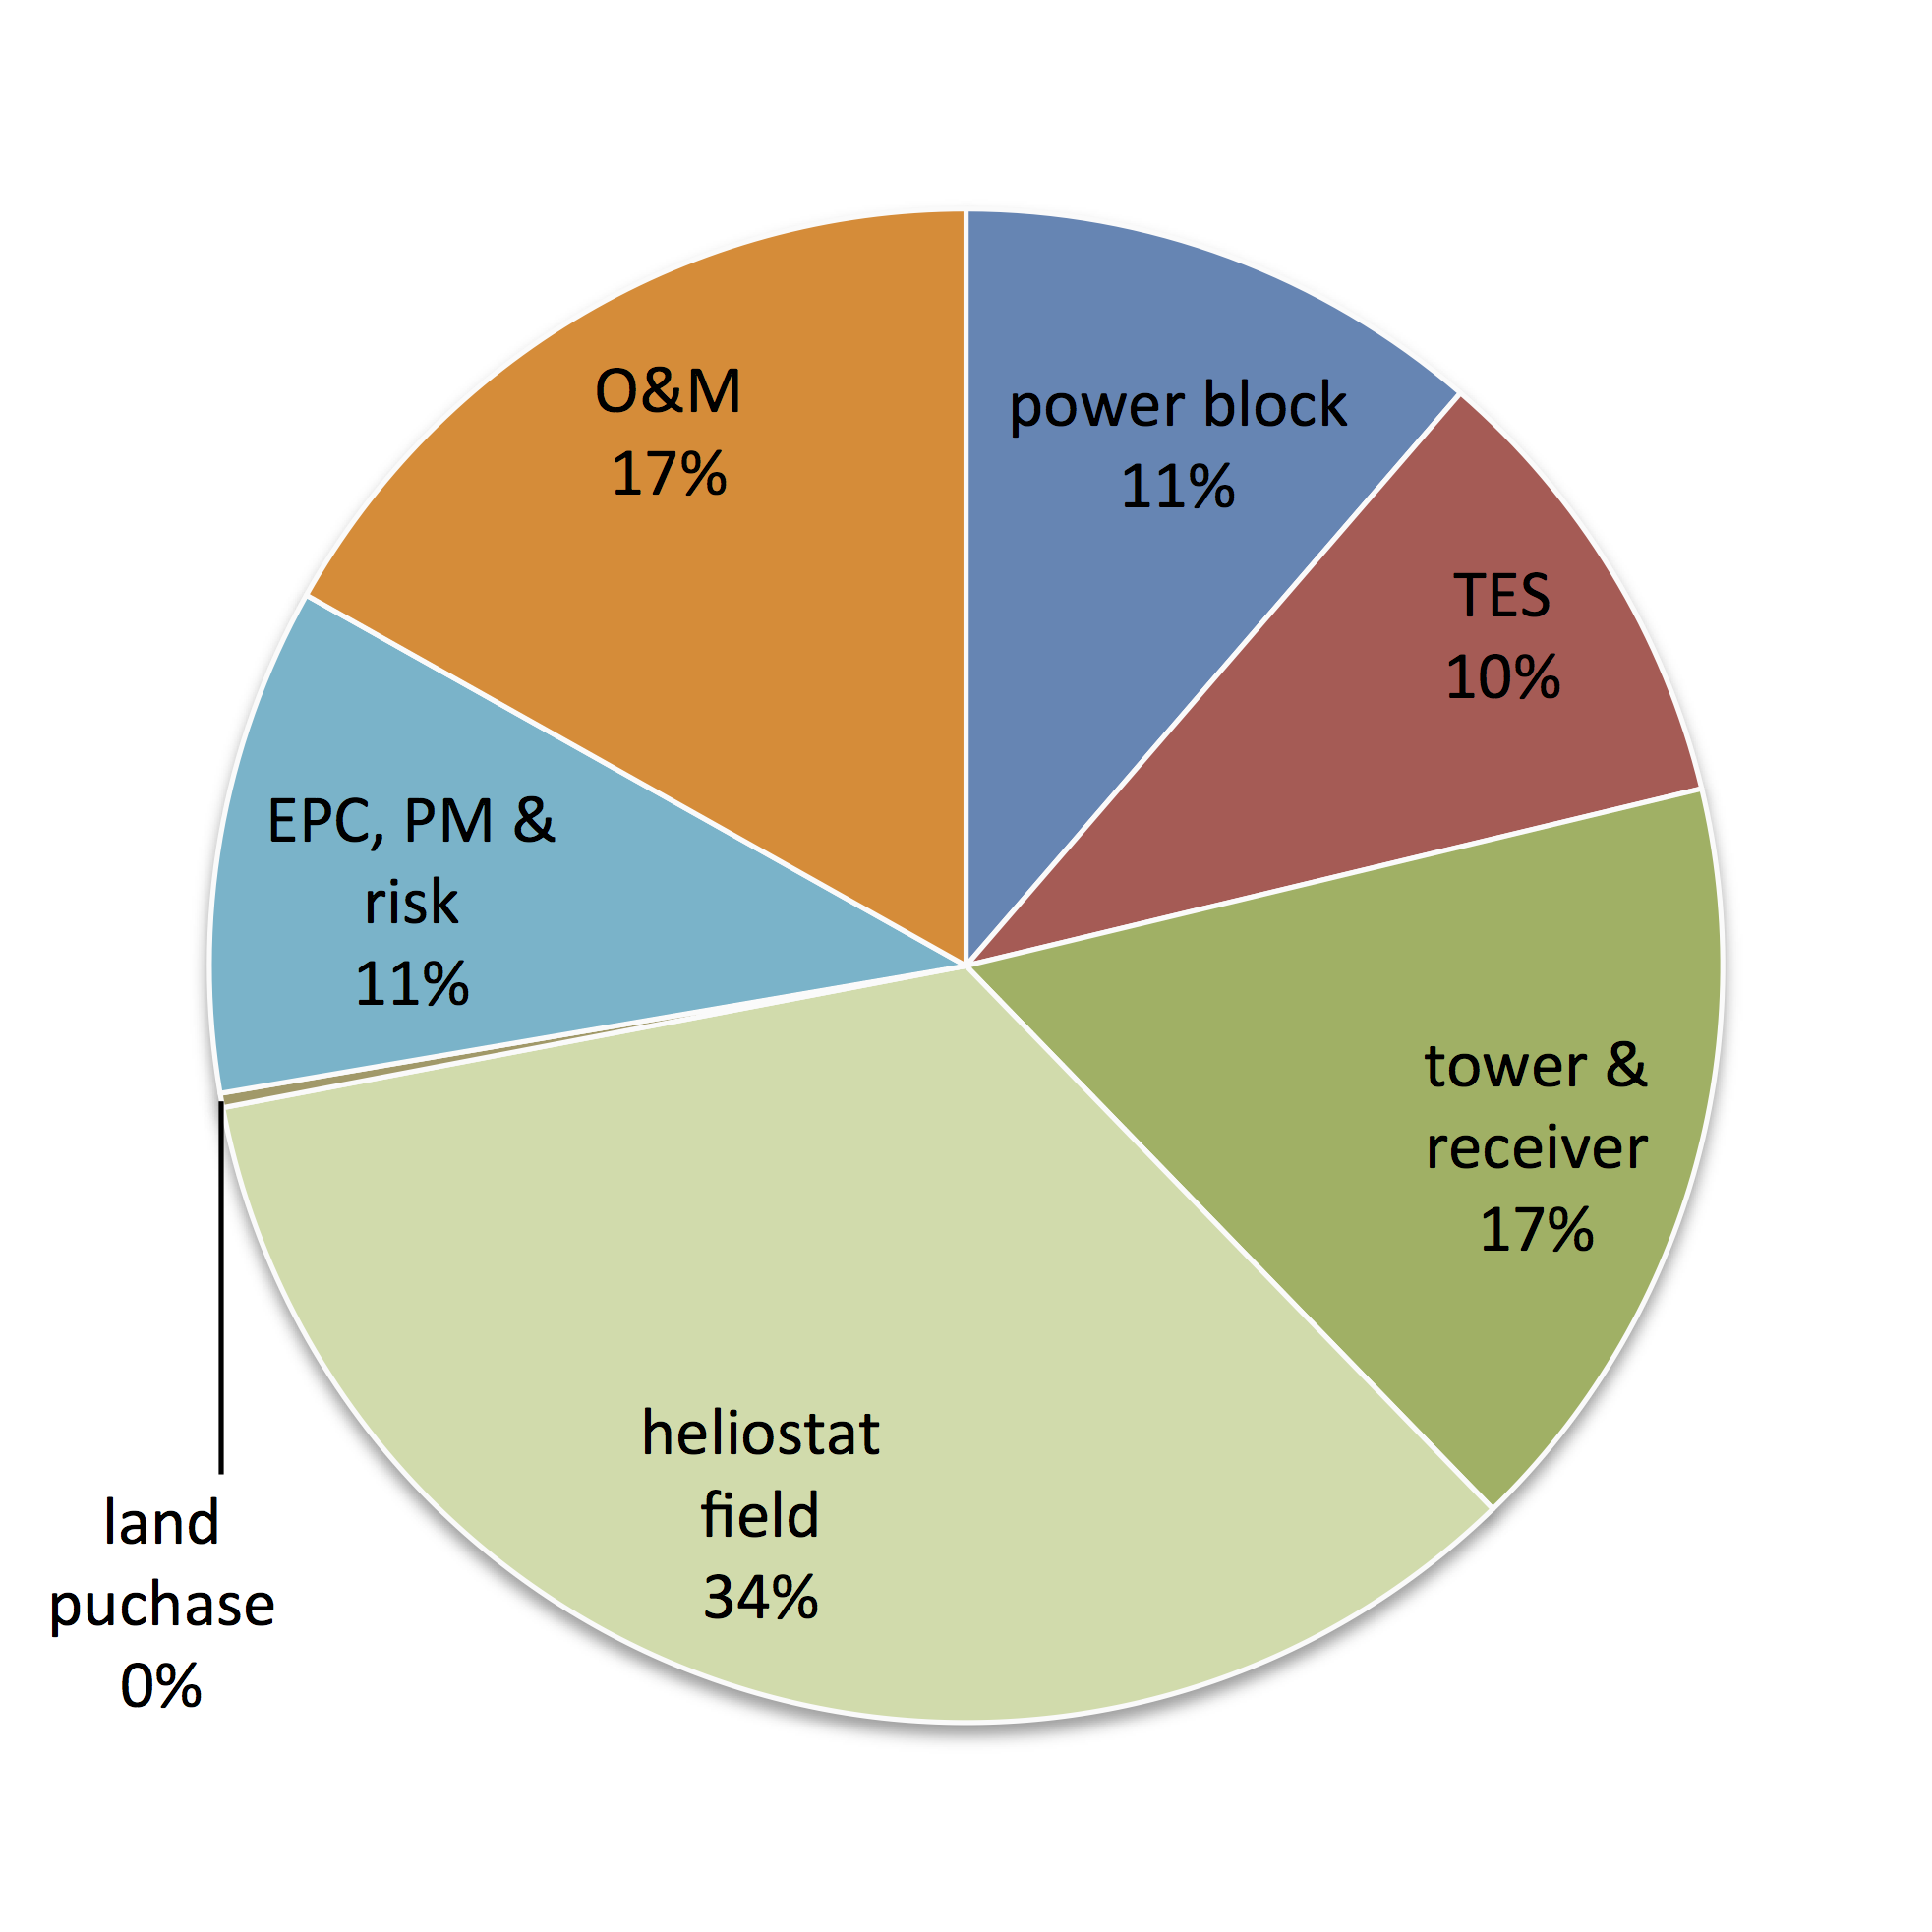
\includegraphics[width=1\textwidth]{FIG/CR_LCOE_90_BreakDown}
                \caption{CR at \SI{90}{\percent} LCC.}\label{CR_LCOE_90_BreakDown}
        \end{subfigure}%
        ~
        \begin{subfigure}[b]{0.5\textwidth}
                \centering
                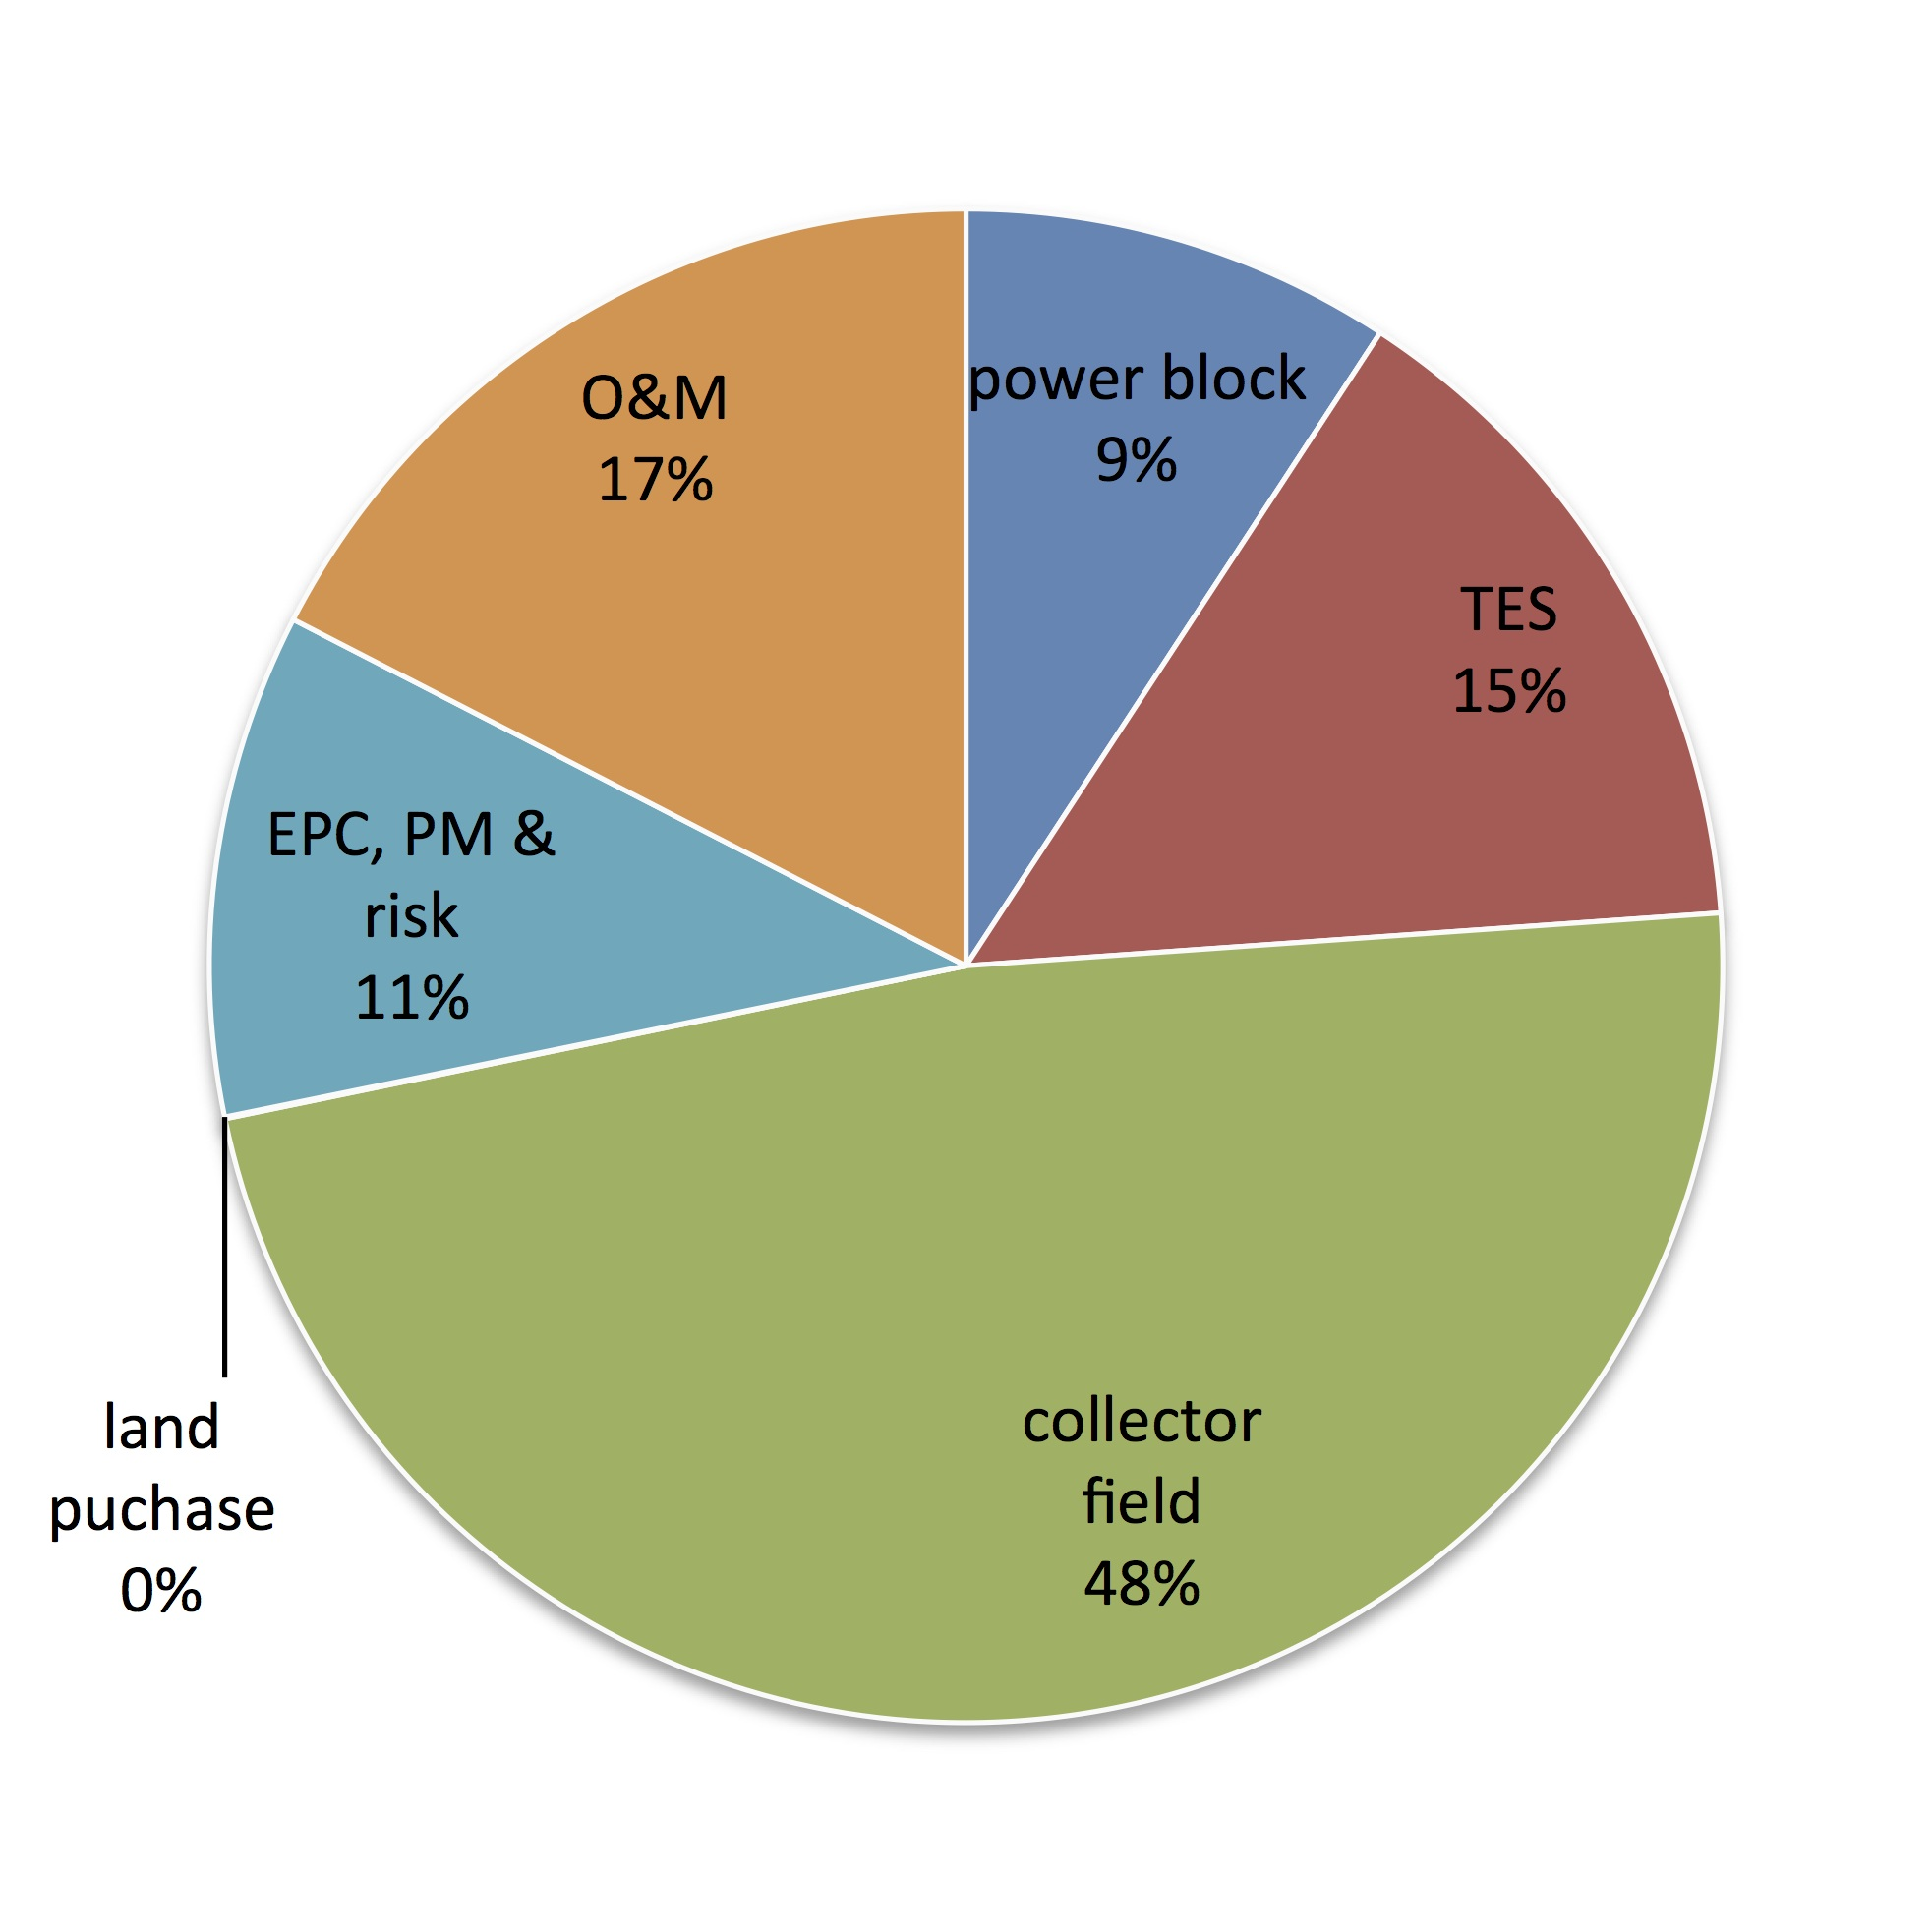
\includegraphics[width=1\textwidth]{FIG/PTC_LCOE_90_BreakDown}
                \caption{PTC at \SI{90}{\percent} LCC.}\label{PTC_LCOE_90_BreakDown}
        \end{subfigure}
\par\medskip % Linebreak   
        \begin{subfigure}[b]{0.5\textwidth}
                \centering
                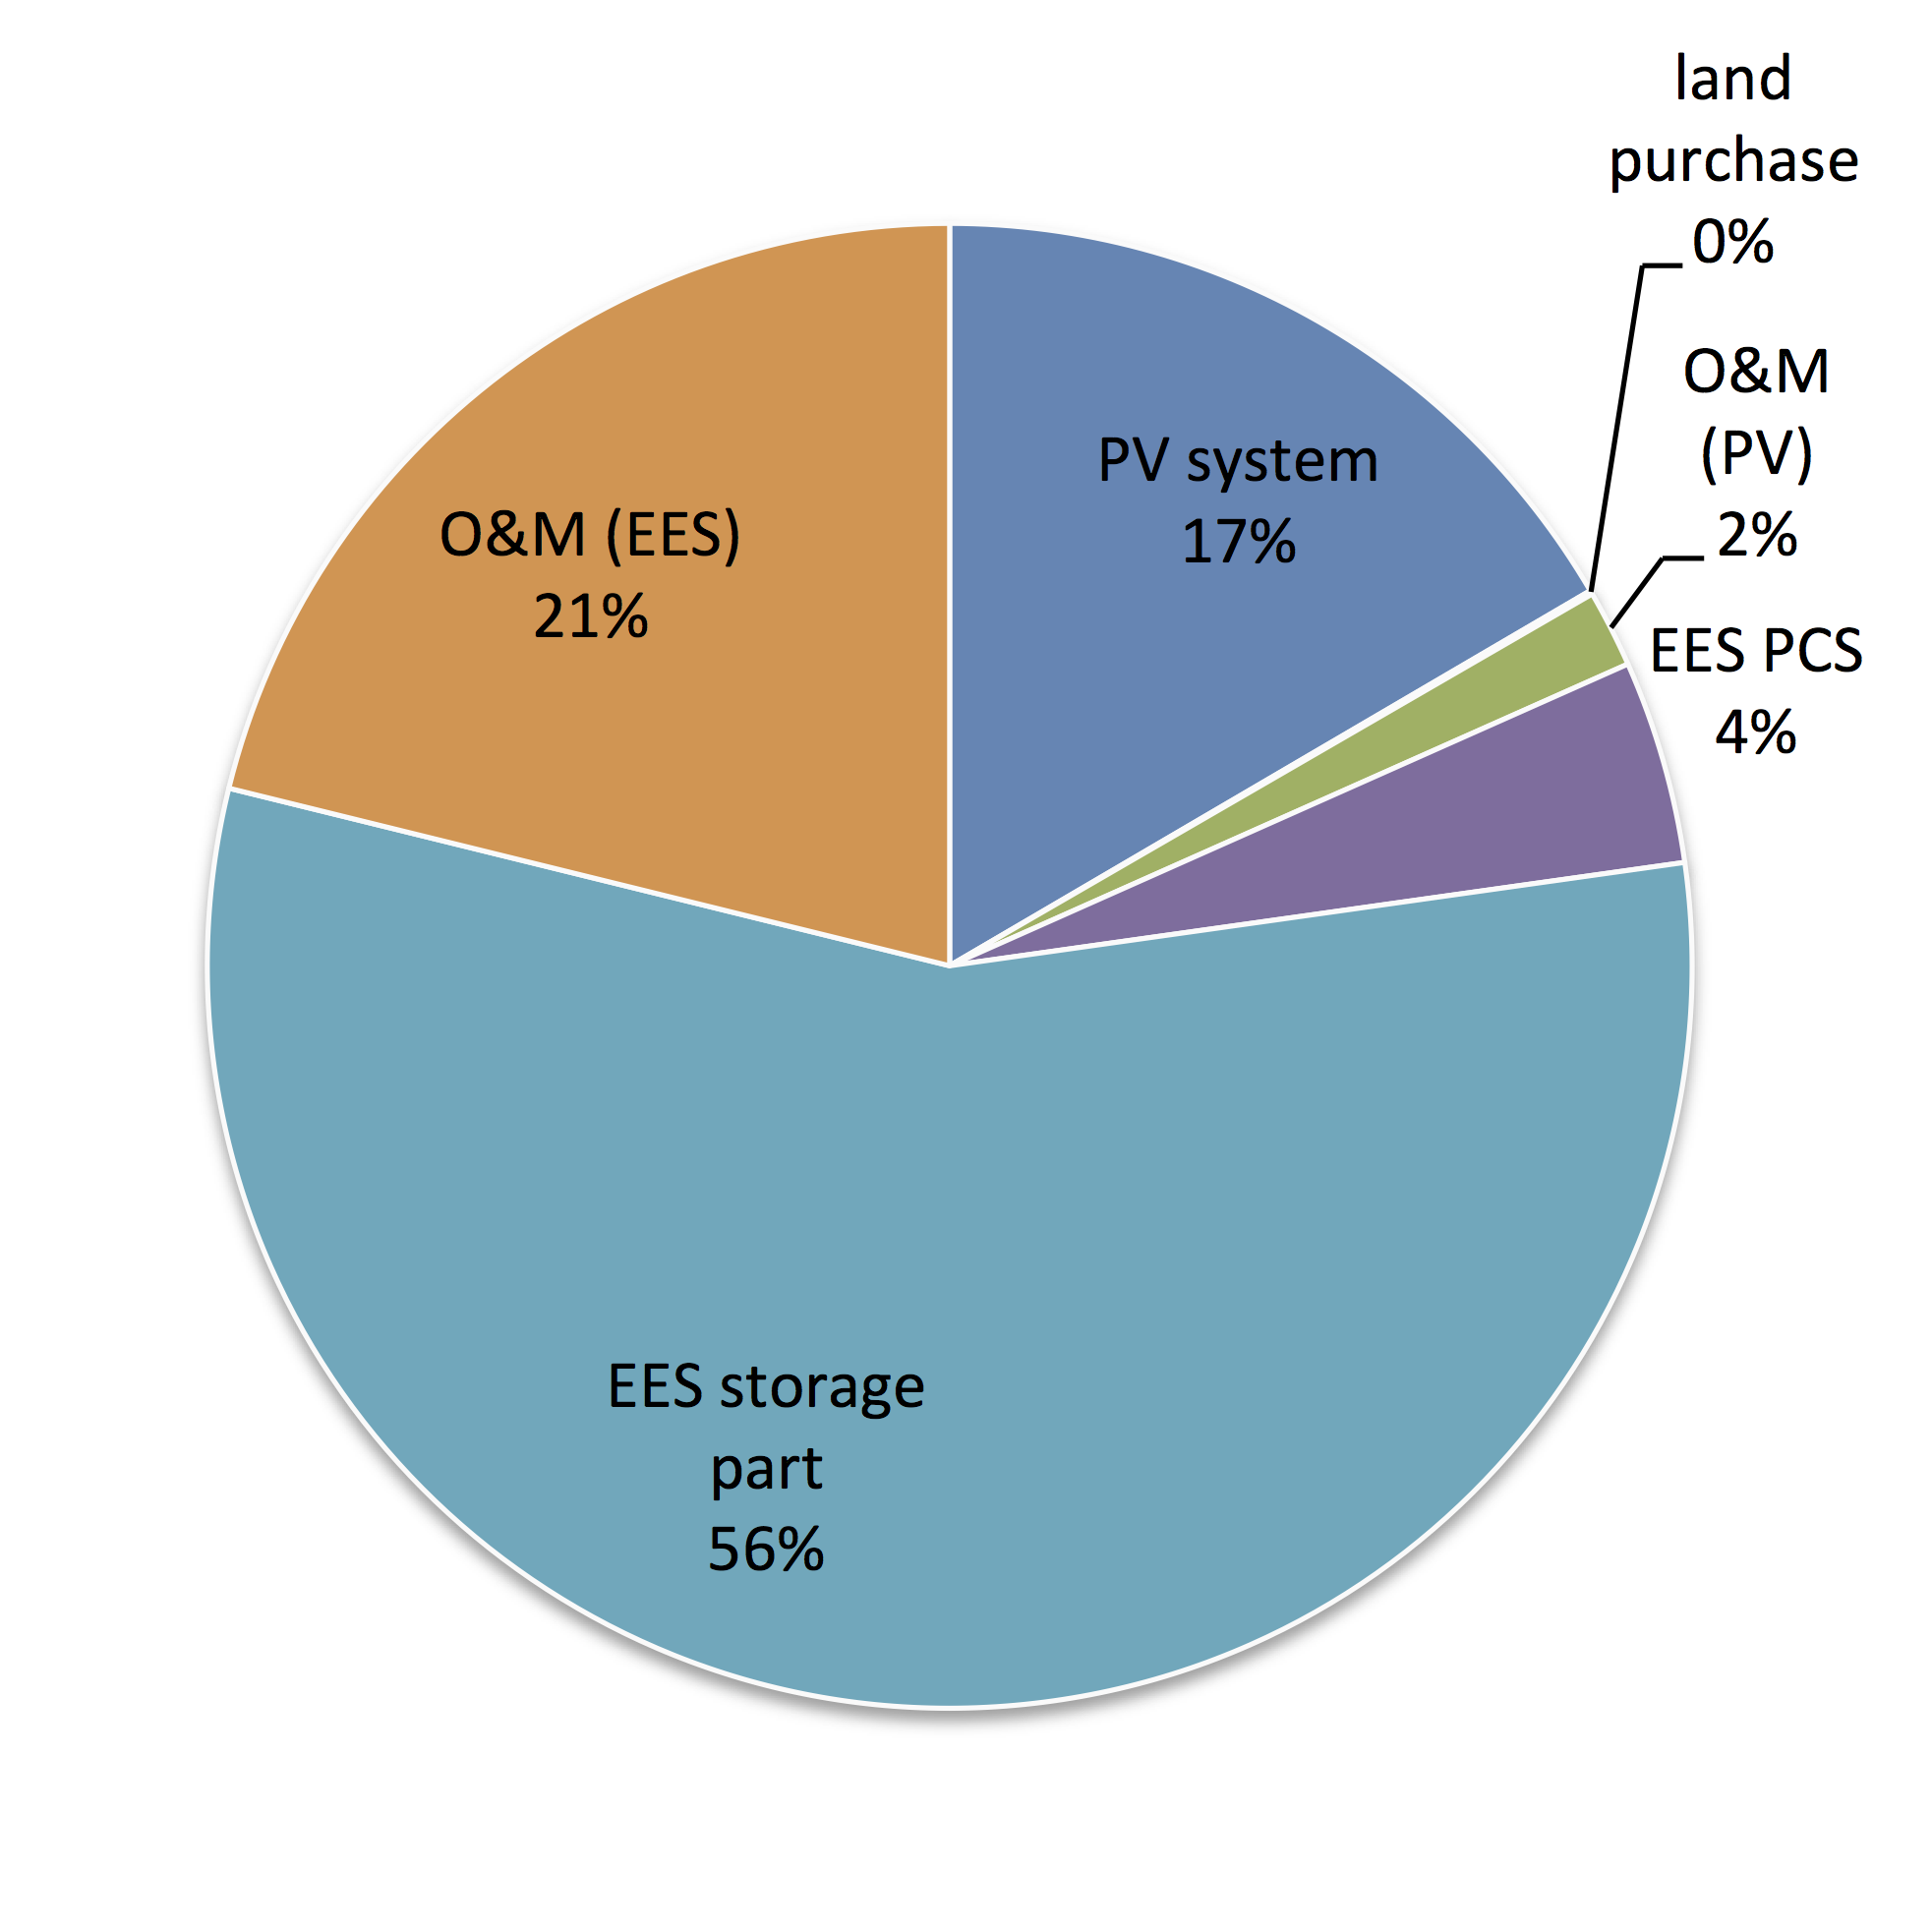
\includegraphics[width=1\textwidth]{FIG/PV_LCOE_90_BreakDown}
                \caption{PV with adapted EES at \SI{90}{\percent} LCC.}\label{PV_LCOE_90_BreakDown}
        \end{subfigure}
        \caption[Break-down of selected LCOE calculation results.]{Break-down of selected LCOE calculation results.}\label{SMPV_LCOE_BreakDown}
\end{figure}
Comparing the LCOE break-down shares (Figure~\ref{SMPV_LCOE_BreakDown}) of the selected simulated solar power plants it shows that the CSP power plants costs are dominated by the concentrating and heat collecting components, while the main cost part of the PV power plant is the EES part. The EES makes more than \SI{80}{\percent} of the PV plants LCOE share. This is a huge share compared with the TES of the CSP plants. It can be seen that the TES of the PTC system has a greater proportion of the costs than in the CR system, which is based in the twice that high specific costs for the storage. The capital cost for land purchase are that low that they has no influence on any simulated solar power plant LCOE. 

The sum of the specific investment costs of the selected CSP plants are with \SI{7503}{USD/kW} for the CR system and \SI{7540}{USD/kW} for the PTC system almost the same. This fits also to the from the IEA predicted average specific investment cost in 2015 with about \SI{7362}{USD/kW} \cite{IEA2014c}. The PV system was calculated with specific investment costs of \SI{1285}{USD/kW} (Page~\pageref{SUBSUBPVFinancialparameter}) which is below the prognosticated cost range of the IEA for large-scale solar PV systems (Figure~\ref{investmentcost}). 

The IEA gives also a prediction for solar power investment cost degradation till 2050. After this prognosis will the specific investment costs of the CSP decrease by about \SI{54}{\percent} and the PV system costs by about \SI{60}{\percent} in total till 2050 \cite{IEA2014c}.

\begin{figure}[htbp]  
\centering
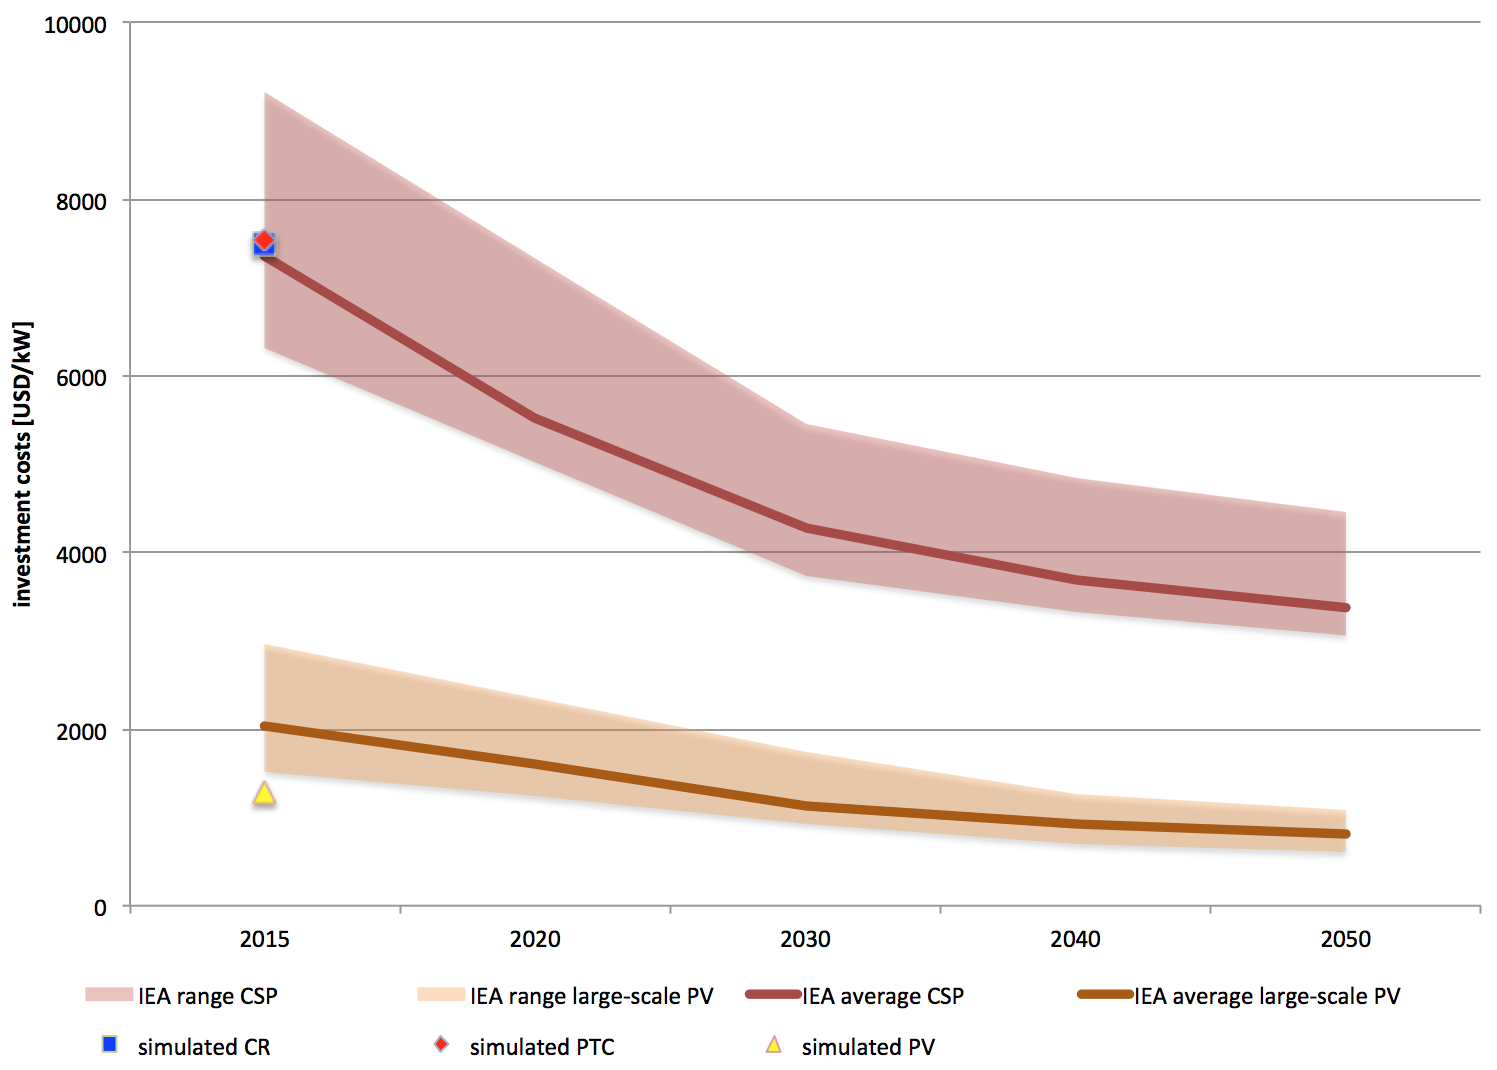
\includegraphics[width=1\linewidth]{FIG/investmentcost}
\caption[Specific investment cost of seleced simulated solar power plants and IEA cost degradation prediction.]{Specific investment cost of seleced simulated solar power plants and IEA cost degradation prediction.}\label{investmentcost}
\end{figure}
As it was shown the costs of the PV power plant with EES is dominated by the cost for the EES storage unit. Nevertheless the assumed specific cost of the Li-ion batteries of \SI{300}{USD/kWh}  (Page~\pageref{SUBSUBPVFinancialparameter}) is comparatively optimistic as it can be seen in Figure~\ref{CostofLi-ion}. But in these publication "Rapidly falling costs of battery packs for electric vehicles" it was shown, that the annual cost reductions for battery storage was about \SI{8}{\percent} the past years which led to the current average battery cost for market-leading actors of \SI{300}{USD/kWh} in 2014 and predicts the costs for 2017-2018 at around \SI{230}{USD/kWh} \cite{Nykvist2015}. It can not be assumed that this high annual cost reductions can be retained over the next decades, but storage costs of \SI{200}{USD/kWh} in 2020, as well as \SI{150}{USD/kWh} in 2030 could be feasible, which confirms also other publications \cite{MckinseyQuaterly2012}.

\begin{figure}[htbp]  
\centering
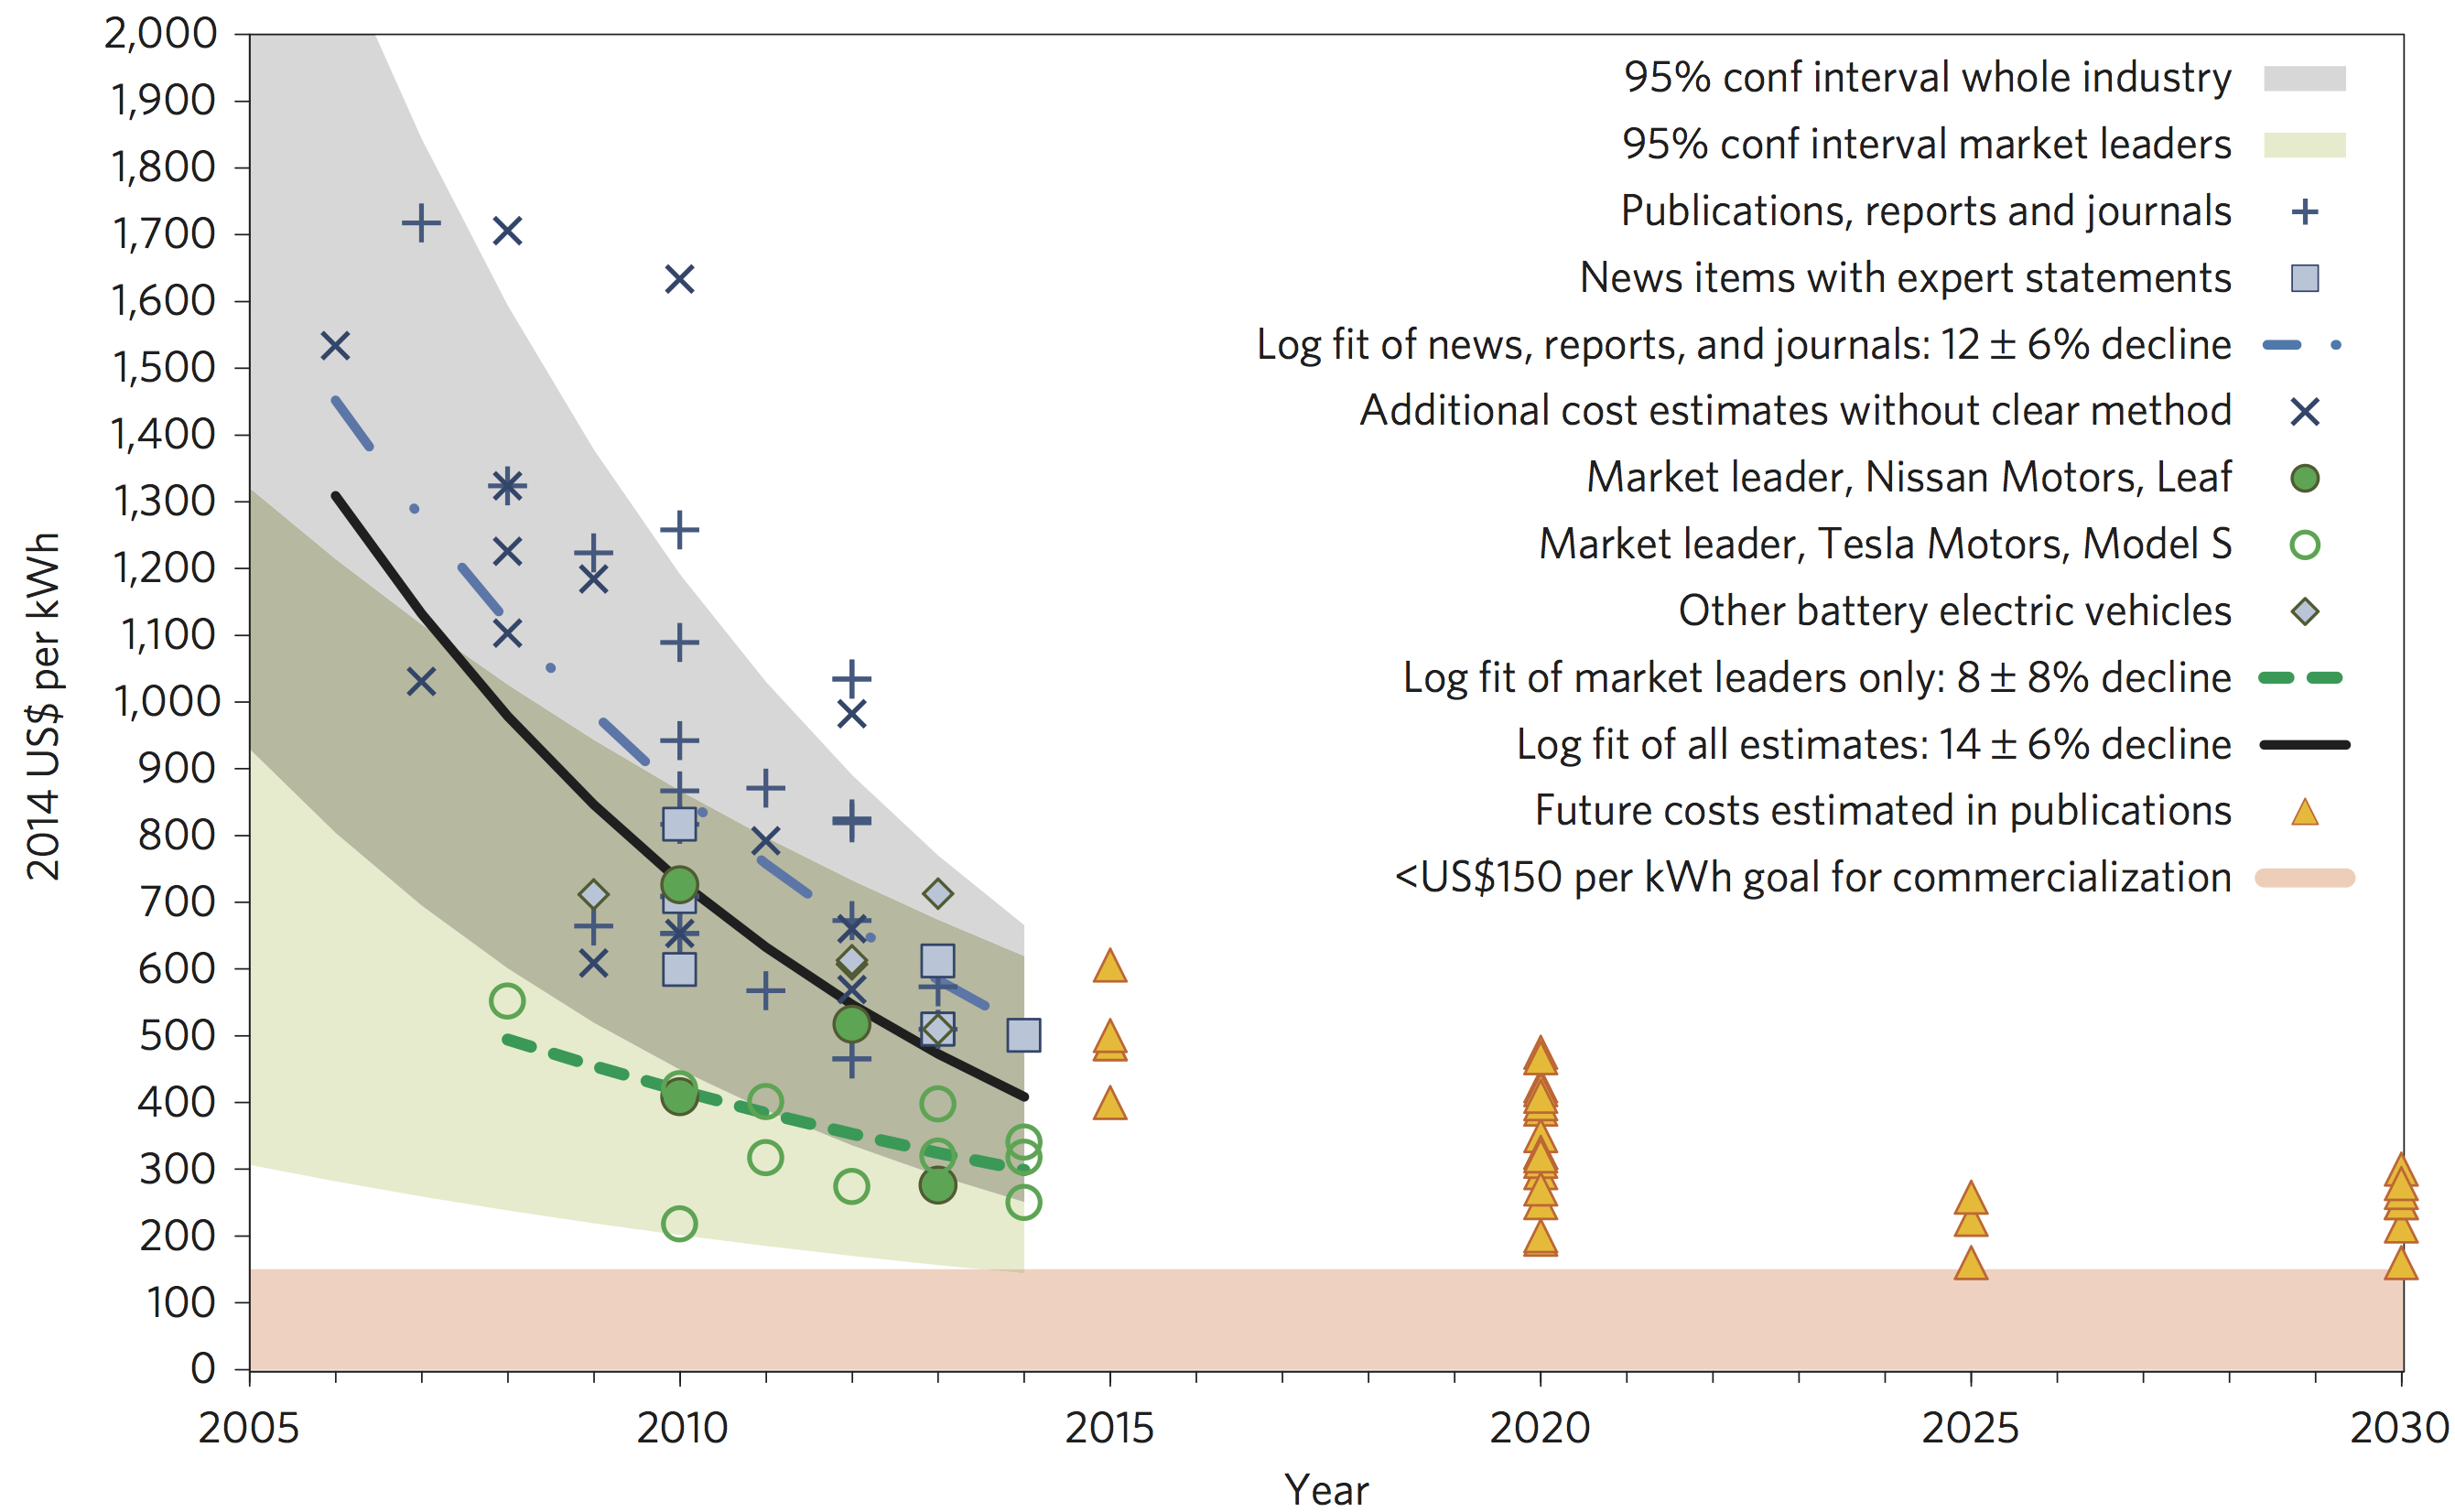
\includegraphics[width=1\linewidth]{FIG/CostofLi-ion}
\caption[Cost of battery packs in battery electric vehicles.]{Cost of battery packs in battery electric vehicles \cite{Nykvist2015}.}\label{CostofLi-ion}
\end{figure}
The estimated cost reduction for the coming decades of solar power applications and EES was used for a medium-term lookout of the LCOE of the selected simulated systems. Figure~\ref{Costdegrad} shows the expected cost development of the selected solar power plants\footnote{Using the average cost reduction behaviour from \cite{IEA2014c} and assumed storage part cost of the EES of \SI{200}{USD/kWh} in 2020 and \SI{150}{USD/kWh} in 2030.} and the currently expected costs per \si{MWh} for new-built conventional power stations\footnote{Costs per \si{MWh} for conventional new-built options as per IRP Update \cite{CSIR2015a} by using a avarage exchange rate from 2014 of \SI{11.286}{USD/ZAR} \cite{IRS2015}.}. 

It can be seen that the reduction of the EES storage part effects the electricity price of the PV power plant with EES enormously and could halved the LCOE by 2030. 

\begin{figure}[htbp]  
\centering
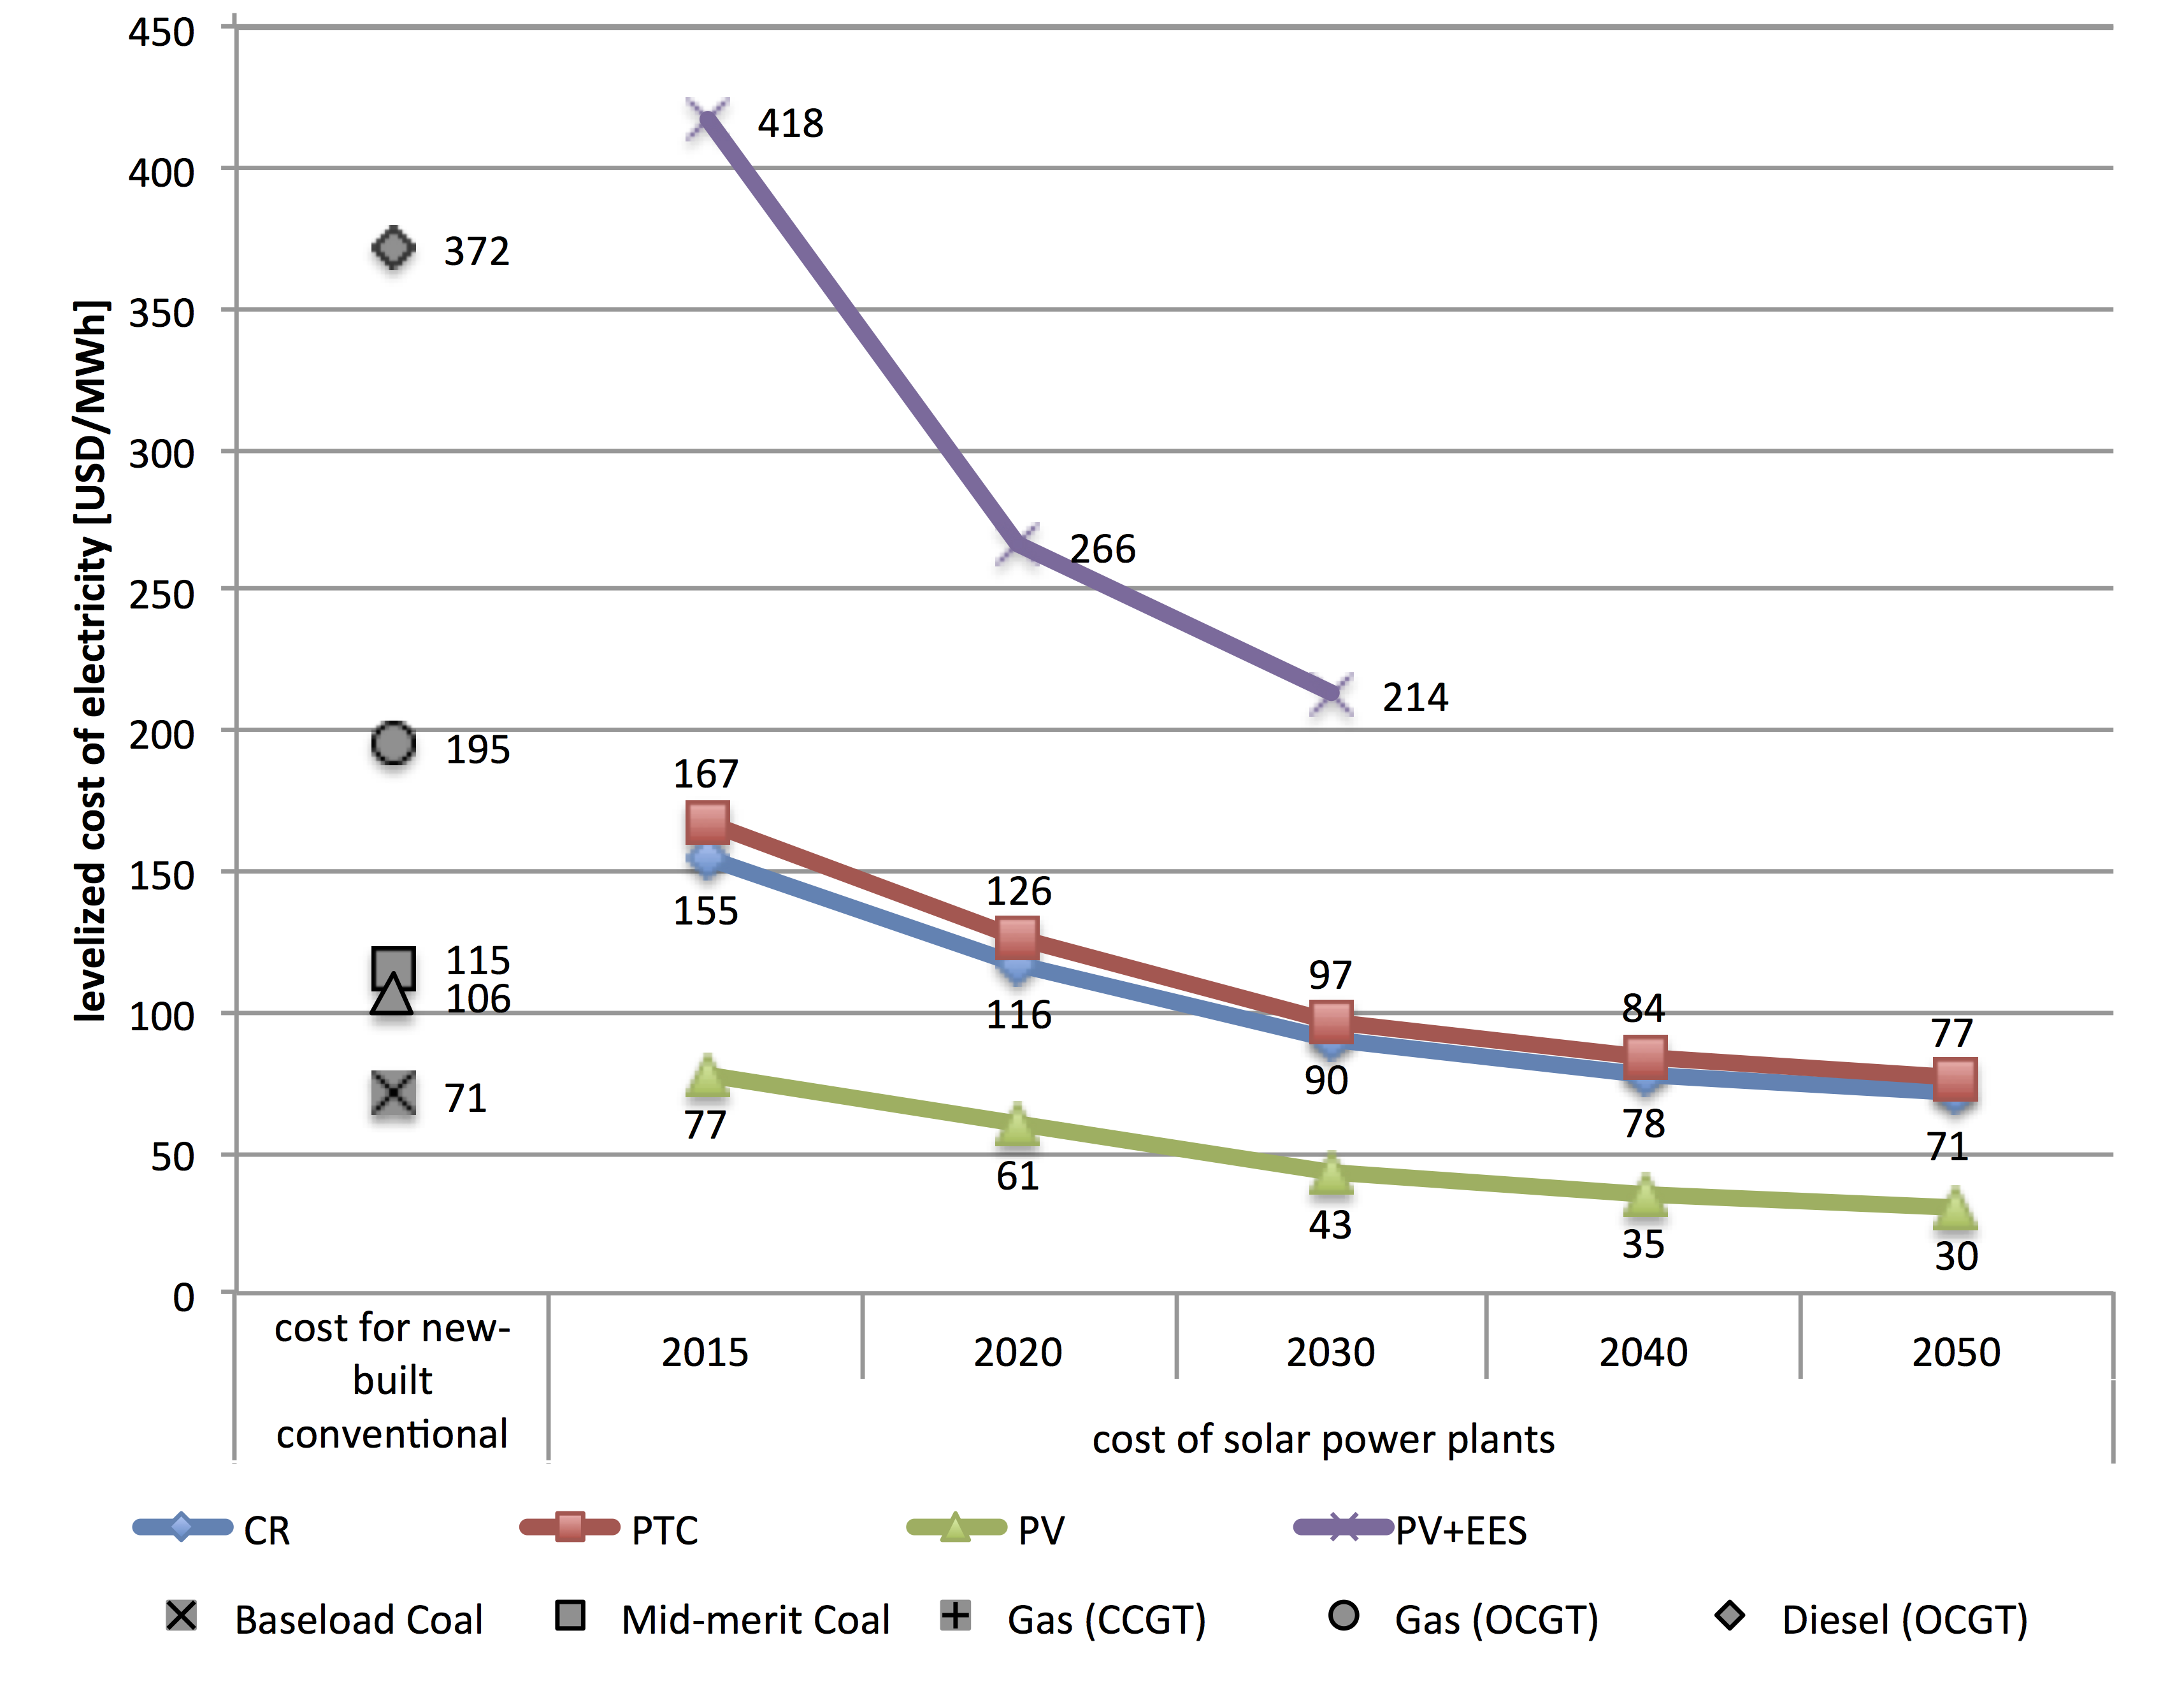
\includegraphics[width=1\linewidth]{FIG/Costdegrad}
\caption[.]{.}\label{Costdegrad}
\end{figure}

EES almost that cheap as Diesel (OCGT)